
% CHAPTER 3

\chapter{METHODOLOGY}
\label{chp:Methodology}


\externaldocument{chapter1}
\externaldocument{chapter2}
\externaldocument{chapter6}
\externaldocument{chapter4}
\externaldocument{chapter5}

In this thesis work, the problem of dynamical formation control of heterogeneous mobile robots is reduced down to two subproblems such as local positioning and formation control.  In our implementation there are two main types of agents in the swarm. First type agents have position measurement sensors on their boards. We call these agents position beacons and only limited number of agents are position beacons in our swarm. Second type agents do not have position sensors on their boards. Local positioning subsystem proposes a solution for the localization of agents in the workspace for second type of agents. On the other hand, formation control subsystem implements algorithms to cover the desired formation shape homogeneously with the agents in the swarm. In this chapter, our solutions for these subproblems are presented in details.

A general block diagram of the system design is illustrated in Figure \ref{general_system}. According to this diagram, local positioning system provides a basis for the formation control problem with agents' state vectors composed of translational positions and velocities. Basically, this subsystem provides position and velocity data to the second type of agents in the swarm. Formation control subsystem proposes a solution to achieve desired complex shapes with heterogeneous agents in the swarm. Formation control system gets the requested formation shape externally and creates individual control laws for agents to cover the desired shape homogenously. The implementation details of these subsystems are given in the following sections. 
\begin{figure}[H]
\caption{General Block Diagram of the Provided Solution} \label{general_system}
\centering
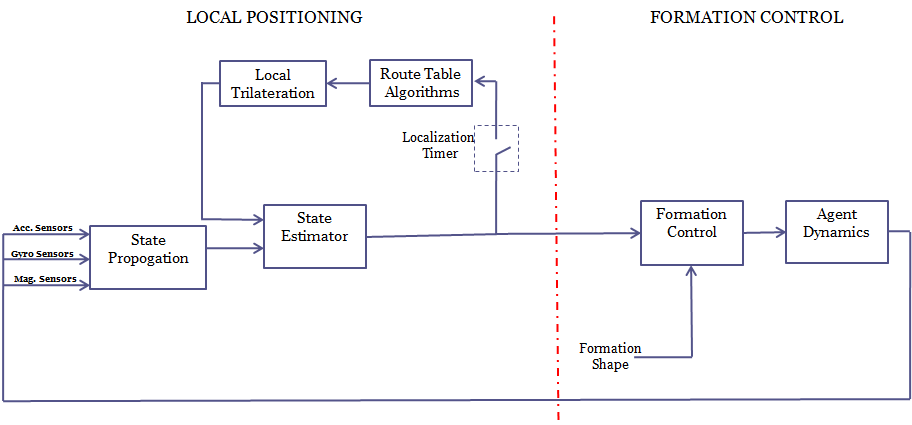
\includegraphics[scale = 0.58]{general_scheme}
\end{figure}

\section{LOCAL POSITIONING SYSTEMS} \label{LOCAL POSITIONING SYSTEMS_ref}
Local positioning system is a subsystem to provide a complete solution to the localization of the second type agents in the workspace. As discussed in Section \ref{Objectives}, agents are expected to have low sensor capabilities and only a limited number of them have external position measurement sensors on their boards and we call these agents position beacons in our project. The rest of the swarm which is composed of second type agents, has to maintain their position$\&$velocity data with the help of their inertial measurements and local trilateration process. Propagation of the states with these inertial measurements are always inclined to drift problems due to the error$\&$noise and bias problems of the sensors \cite{91}. Because of this problem, we have corrected these state vectors with an external measurement provided by local trilateration process. We have proposed a complete solution for this subsystem as illustrated in Figure \ref{figure_lps}.

\begin{figure}[H]
\caption{Local Positioning System} \label{figure_lps}
\centering
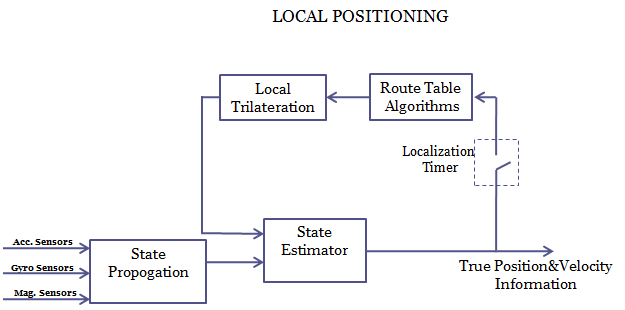
\includegraphics[scale = 0.65]{lps}
\end{figure}

As illustrated in Figure \ref{figure_lps}, agents propagate their states with the help of inertial measurements. This state propagation process is executed with high speed data provided by the inertial sensors. On the other hand, trilateration and route table determination processes require iterative and time consuming algorithms and their implementation details are given in the following sections. It is not possible to execute the trilateration and route table determination algorithms with the same execution frequency of state propagation process. Because of this reason, a localization timer to provide the minimum required time for the route table determination and trilateration process is implemented to the solution. Agents will correct their state vectors with the localization period by measuring their positions with trilateration process and execute the update procedure in their state estimator algorithms. The requirement about the maximum value of the localization period is determined with the help of Monte Carlo simulations discussed in Section \ref{lps_ref} by defining a maximum allowable error on the position data. 

Local trilateration process requires distance measurements to the position beacons which are direct neighbors of an agent. Route table algorithms are used to provide information to the agents about the position beacons whether they are direct neighbors or not. On the other hand, route tables also implement a mesh network between agents. This network is used to transport data globally over the network. It is composed with a bidirectional graph in which each agent can communicate with its direct neighbors. In this graph, we have assigned an edge between two nodes if there is a radio link between them. This line of sight(LOS) radio link is the main criteria for the agents to become direct neighbors in the network. Thus, having a physical Euclidian distance to an agent within the communication range is not enough to be the direct neighbor with that agent, i.e. even if two agents are very close to each other in the workspace, they are not direct neighbors if there is no radio link between them because of an obstacle preventing the line of sight. Figure \ref{sample_mesh} shows an example of a mesh network created with 8 agents in the environment.

\begin{figure}[H]
\caption{A Sample Mesh Network Created with 8 Agents} \label{sample_mesh}
\centering
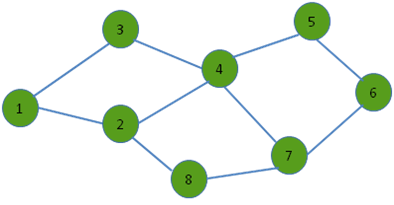
\includegraphics[scale = 0.58]{mesh}
\end{figure}
 
\subsection{Local Trilateration Process}
Trilateration process helps the second type agents to localize themselves with the help of position beacons which are their direct neighbors.  Trilateration calculations use distance measurements to the position beacons with known positions, to determine the coordinates of second type agents \cite{22}. These measurements are assumed to be done with the help of time of arrival(TOA) methods as discussed in Section \ref{sssec:num1}. In a TOA solution, an agent is able to measure the distance from itself to a position beacon only if it is a direct neighbor of that position beacon. Figure \ref{beacons_ref} illustrates simulation environment of a swarm which includes 5 position beacons. Here agent $C$ tries to localize itself with the help of distance measurements $r_i$ and the position data $B_i$ of the position beacons. It has 4 position beacons as direct neighbors in the network and this information is provided by the route table of agent $C$ as defined in Section \ref{route_route}.

\begin{figure}[H] 
\caption{Environment for Trilateration Process} \label{tri_late}
\centering
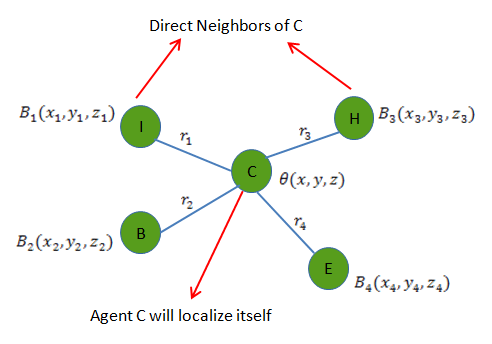
\includegraphics[scale = 0.55]{beacons}
\label{beacons_ref}
\end{figure}

For the simulation environment illustrated in Figure \ref{tri_late}, the distance function to any position beacon can be written as follows \cite{22};

\begin{equation} % eq 2
{r_i} = \sqrt{(x-x_i)^2 + (y-y_i)^2+ (z-z_i)^2}    \hspace{0.3cm}   (i=1,2,...,n)
\end{equation}

where $i$ denotes the beacon number and $n$ is the total number of position beacons which is equal to 4 in our case.  In general, we have $n$ number of constraints in the solution of the localization problem. These constraints are defined as spherical functions for a localization problem in 3 dimensional workspace \cite{22}. In our work, we have implemented a two dimensional localization solution with the assumption of each agent of the swarm conserve the same vertical position within the Earth centered coordinate system. With this assumption, the problem for the localization process has constraints with circle functions rather than spherical ones, presented with

\begin{equation}
(x-x_i)^2 + (y - y_i)^2 = {r_i}^2 \hspace{0.3cm}   (i=1,2,...,n)
\end{equation}

It is possible to use these $n$ circular constraints to calculate the unknown position of the agent $C$. For this purpose, lets assume $\theta = (x,y)$ is representing the coordinates of agent $C$ and $B_1 = (x_1,y_1) ; B_2 = (x_2,y_2) ; B_3 = (x_3,y_3) ; ...  ; B_i = (x_i,y_i)$ are the measured positions of the position beacons.

If any of these beacons is considered as the reference beacon and named with an index of $r$, the distance equations can be provided as following:

The distance between the agent $C$ and any beacon $i$ represented as

\begin{equation} \label{3.3}
d_i(\theta) = \sqrt{\left((x - x_i)^2 + (y - y_i)^2\right)}
\end{equation}

The distance between the reference beacon which is located at $B_r = (x_r,y_r)$ and the other beacons is evaluated as

\begin{equation}
d_{ir}(\theta) = \sqrt{\left((x_i - x_r)^2 + (y_i - y_r)^2\right)}
\end{equation}

The distance between the agent $C$ and the reference beacon is obtained as

\begin{equation}
d_r(\theta) = \sqrt{\left((x - x_r)^2 + (y - y_r)^2\right)}
\end{equation}

Adding and subtracting $x_r, y_r$ and $z_r$ in equation \ref{3.3} gives

\begin{align} \label{tri_expressi}
\begin{split}
d_i^2(\theta) = & (x - x_r + x_r - x_i)^2 + (y - y_r + y_r - y_i)^2 \\ 
              = & (x - x_r)^2 + 2(x_r - x_i)(x - x_r) + (x_r-x_i)^2 \\
              + & (y - y_r)^2 + 2(y_r - y_i)(y - y_r) + (y_r - y_i)^2
\end{split}
\end{align}

Replacing the expressions in equation \ref{tri_expressi} by $d_{ir}$ and $d_r$, the equation can be written as:

\begin{equation}
 2((x_i - x_r)(x - x_r) + (y_i - y_r)(y - y_r)) = d_r^2(\theta) + d_{ir}^2 - d_i^2(\theta)
\end{equation}

this general expression is valid for each beacon with $i$ changing from $2$ to $n$ (by assuming that we have chosen the first position beacon with $"r=1"$ as reference beacon)

\begin{align}
\begin{split}
& (x_2 - x_1)(x - x_1) + (y_2 - y_1)(y - y_1) = \frac{1}{2} [d_1^2(\theta) + d_{21}^2 - d_2^2(\theta)] \\
& (x_3 - x_1)(x - x_1) + (y_3 - y_1)(y - y_1) = \frac{1}{2} [d_1^2(\theta) + d_{31}^2 - d_3^2(\theta)] \\
& ... \\
& (x_n - x_1)(x - x_1) + (y_n - y_1)(y - y_1) = \frac{1}{2} [d_1^2(\theta) + d_{n1}^2 - d_n^2(\theta)]
\end{split}
\end{align}

if $b_{ir}$ is defined for each beacon as follows:

\begin{equation}
b_{ir} := \frac{1}{2}[d_r^2(\theta) + d_{ir}^2 - d_i^2(\theta)]
\end{equation}

then the linearized system equations can be represented with $A\vec{x} = \vec{b}$ type equation where;

\begin{equation}
A = \begin{bmatrix}
x_2 - x_1 & y_2 - y_1\\
x_3 - x_1 & y_3 - y_1\\
...       & ...      \\
x_n - x_1 & y_n - y_1\\
\end{bmatrix}				
\end{equation}

\begin{equation}
x = \begin{bmatrix}
x - x_1\\
y - y_1\\
\end{bmatrix}
\end{equation}

\begin{equation}
b = \begin{bmatrix}
b_{21}\\
b_{31}\\
... \\
b_{n1}\\
\end{bmatrix}
\end{equation}

with $A$ is a $(n-1)\ x\ 2$ matrix and $b$ is a $(n-1)\ x\ 1$ vector.

There are some possible solutions to this type of equation regarding with the structure of matrix $A$ and vector $b$.\\

\underline {\textit{Solution to $A\vec{x} = \vec{b}$ Problem}}\\
In a localization problem handled in two dimensional space, the $A$ matrix has $(n-1)$ rows and $2$ columns, where $n$ is the number of position beacons which are direct neighbors of an agent. There is no solution when the number of neighbors lower than $3$ (i.e. $n<3$) \cite{22}. When the number of neighbor position beacons are equal or greater than $3$ we have three different solutions according to the structure of the linearized equations.

\textit{1) Unique Solution:}\\
 If A is a $2\ x\ 2$ matrix (i.e. $n=3$) and the its rank is $2$, then the solution of $\vec{x}$ is unique with \cite{linear_ders_notu}

\begin{equation}
\vec{x} = A^{-1}\vec{b}
\end{equation}

where $\vec{x}$ is the unique solution. \\
  
\textit{ 2) Minimum Norm Solution With Pseudo Inverse:} \\  
If $A$ is a $(n-1)\ x\ 2$ dimensional matrix where $n>3$ ,which means the number of neighboring position beacons greater than $3$, and if columns of $A$ matrix form a linearly independent set (full column rank matrix) then the solution can be found with the projection of $\vec{b}$ over range space of $A$, $Proj_{R(A)}\vec{b}$ where \cite{linear_ders_notu}

\begin{equation}
Proj_{R(A)}\vec{b} = A (A^TA)^{-1}A^T\vec{b}
\end{equation}

\begin{align}
\begin{split}
& A\hat{x} = Proj_{R(A)}\vec{b}\\
& A\hat{x} = A(A^TA)^{-1}A^T\vec{b}
\end{split}
\end{align}
 
We can justify this expression by passing the righthand side term to the left

\begin{equation}
 A(\hat{x} - (A^TA)^{-1}A^T\vec{b}) = 0
\end{equation}

then 

\begin{equation}
\hat{x} = (A^TA)^{-1}A^T\vec{b}
\end{equation}
  
$(A^TA)$ is invertible since $A$ matrix is full column rank matrix, so 

\begin{align}
\begin{split}
\mathcal{N}(\mathbf{A}) = \{0\} \hspace{0.3cm}  and  \hspace{0.3cm}  \mathcal{N}(\mathbf{A})^\perp =\mathbb{R} ^n 
\end{split}
\end{align}
  
then 
  
\begin{equation}
Proj_{ \mathcal{N}(\mathbf{A})^\perp}\hat{x} = \hat{x}
\end{equation}
  
this concludes that $\hat{x}$ is the unique minimum norm solution to the $A\vec{x} = \vec{b}$ problem\\
	
	
\textit{3) Minimum Norm Solution with Newton Iteration Method}\\	
If matrix $A$ has the dimensions of $2\ x\ 2$ or $(n-1)\ x\ 2$ with $n>3$ and if rank of $A$ matrix is equal to $1$ then the solution to the $A\hat{x} = \vec{b}$ problem can be found iteratively with the help of nonlinear least squares method that minimizes the cost function which is defined as sum of squares of the distance errors \cite{22} :
	
\begin{equation} \label{cost_func_tri}
F(\theta) = \sum_{i=1}^{n} \left(f_i^2(x,y)\right)
\end{equation}
	
with
	
\begin{equation}
f_i(x,y) = \sqrt{(x-x_i)^2 + (y - y_i)^2} - r_i = f_i(\theta) 
\end{equation}

where $r_i$ is the measured distance to a position beacon $i$ and $(x_i, y_i)$ is calculated position data of agent $C$ iteratively.

There are various algorithms to minimize the cost functions in the literature. We have used Newton iteration to find the optimal solution in this thesis work. Because convergence of this method is quadratic in general and the performance of the algorithm is extremely increased by choosing proper initial conditions \cite{wiki_newton}. We have used the propagated position data as an initial condition for the optimization process to make the algorithm terminated very fast with correct results. Algorithm is implemented as follows:

Considering  $f(\theta)$ as

\begin{equation}
f(\theta) = \begin{bmatrix}
f_1(\theta) \\
f_2(\theta) \\
...         \\
f_n(\theta)
\end{bmatrix}
\end{equation}


We have defined the Jacobien matrix as follows:

\begin{equation}
J(\theta) = \begin{bmatrix}
\frac{\partial{f_1(\theta)}}{\partial{x}} & \frac{\partial{f_1(\theta)}}{\partial{y}} \\
\frac{\partial{f_2(\theta)}}{\partial{x}} & \frac{\partial{f_2(\theta)}}{\partial{y}} \\
... & ... \\
\frac{\partial{f_n(\theta)}}{\partial{x}} & \frac{\partial{f_n(\theta)}}{\partial{y}} \\
\end{bmatrix}
\end{equation}

	
Suppose we are trying to find the position of an agent defined with the vector of $\vec{R}$	
\begin{equation}
 \vec{R} = \left(\begin{matrix}
  x \\ y 
 \end{matrix}\right)
\end{equation}

To optimize the cost function, Newton iteration is implemented as follows;

\begin{equation}
 \vec{R}_{\{k+1\}} =  \vec{R}_{\{k\}} - (J^T_{\{k\}}J_{\{k\}})^{-1}J^T_{\{k\}}\vec{f}_{\{k\}}
\end{equation}	

where $\vec{R}_{\{k\}}$, $J_{\{k\}}$ and $\vec{f}_{\{k\}}$ denotes the variables calculated at $k^{th}$ iteration. The explicit form of the equations can be derived as follows;
	
\begin{equation}
J^TJ = \left(\begin{matrix}
\sum_{i=1}^{n} \frac{(x-x_i)^2}{(f_i+r_i)^2} &  \sum_{i=1}^{n} \frac{(x-x_i)(y-y_i)}{(f_i+r_i)^2} \\
\sum_{i=1}^{n} \frac{(x-x_i)(y-y_i)}{(f_i+r_i)^2} &  \sum_{i=1}^{n} \frac{(y-y_i)^2}{(f_i+r_i)^2}
\end{matrix}\right)
\end{equation}	

and 

\begin{equation}
J^T\vec{f} = \left(\begin{matrix}
\sum_{i=1}^{n}\frac{(x-x_i)f_i}{(f_i+r_i)} \\
\sum_{i=1}^{n}\frac{(y-y_i)f_i}{(f_i+r_i)}
\end{matrix}\right)
\end{equation}
	
	
\subsection{Route Table Determination} \label{route_route}
We have implemented a localization solution in which each second type agent is getting in trilateration process with the position beacons in the swarm as we have introduced previously. It is needed to be direct neighbors of the position beacons to get in trilateration process. In our project, route tables are used to provide information to the agents about the position beacons whether they are direct neighbors or not. On the other hand, they are used to create a mesh network in the swarm to provide a communication backbone. With this mesh network it is possible to send any data globally over the network to any destination by using agents as relays to transmit the data. In our implementation, each agent had its own route table in the network. These route tables include the information about the next nodes and costs to any destination in the network. Next nodes are representing the node which the data will be transferred next for that destination and costs are representing the minimum number of hops (i.e. number of relay agents on the path) for that destination. We have used the cost information for the position beacon destinations to check whether the agent is direct neighbor of that position beacon or not. In other words, the cost to a position beacon is equal to 1 in the route table, if that agent is the direct neighbor of the position beacon


	
\subsubsection{Routing Algorithm- Bellman Ford}
As mentioned in the Section \ref{Objectives}, agents are assumed to have a limited communication range and bandwidth and the communication topology in the swarm must be implemented with a wireless mesh network. In this type of topology, each agent is a relay in the network and the data is transferred to the related destination with the help of route tables. This makes it possible to have the capability of transferring low bandwidth data through the network with multiple hops.  In this work, we have implemented this topology with a table driven routing scheme known as Bellman Ford algorithm. Bellman Ford is an algorithm that computes the shortest paths between any two node in a weighted graph \cite{wiki_bellman}. It has a drawback related with the routing loop problem which occurs in an event of one or more nodes in the graph are lost during the process. The probability of vanishing vertices during the execution of the algorithm is very high since the agents in the swarm have a small range of communication and have a great possibility to lose their connection with the rest of the swarm. For this reason we have implemented an extension of the Bellman Ford algorithm known as Destination-Sequenced Distance Vector Routing Protocol(DSDV) algorithm.  
	
\begin{figure}[H]
\caption{Costs for Shortest Paths to Each Nodes from Agent 'B'} \label{bellman_ref}
\centering
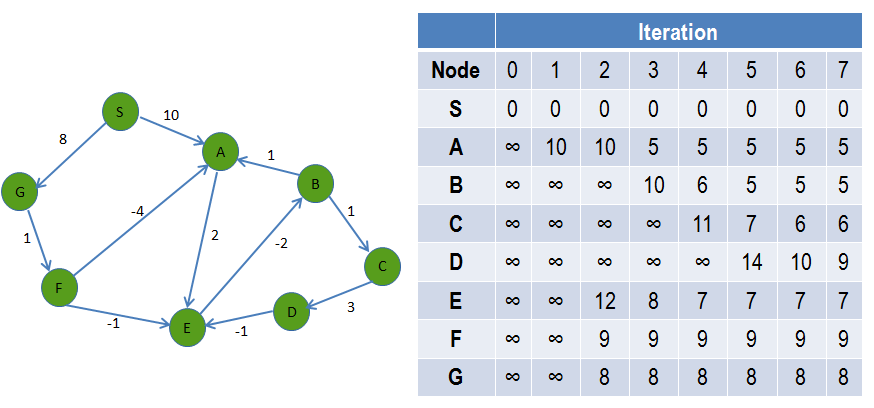
\includegraphics[scale = 0.50]{bellman}
\end{figure}

A simulation of the DSDV algorithm with a simple robot network in our problem is given in the Figure \ref{bellman_ref}. The algorithm to calculate the shortest paths from agent `B` to each destination on network, terminates at the end of 3 iterations. At the beginning of the process, the costs for each destinations are determined as infinitive. Then the shortest paths to the each agent in the given bidirectional graph are determined iteratively with the help of the DSDV algorithm. Since we have defined the shortest paths with the number of hops to each destination, we have used unit weight for each edge in the graph representing the cost of each hop while getting the related destination in the network is equal to 1. 

We have implemented DSDV algorithm to solve the routing problem in the mesh network. Figure \ref{routing_problem2} shows a simulation output illustrating routing loop problem.

\begin{figure}[H] 
\caption{Routing Problem Engaged by a Lost of a Node in Network} \label{routing_problem2}
\centering
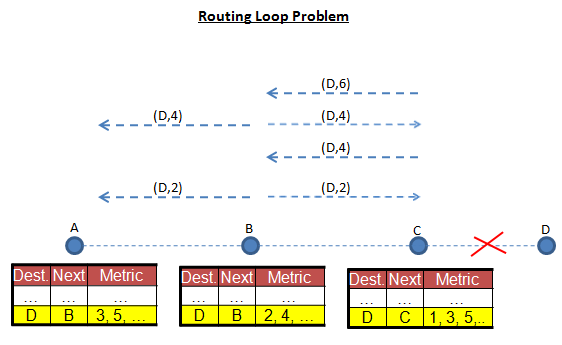
\includegraphics[scale = 0.65]{routing_problem}
\end{figure}

Suppose that agent D has lost its contact with the network due to some malfunction or by being lost wandering outside of the communication range of its closest neighbor. Before this event, agent C had a unit distance to agent D and consequently agent B had a 2 unit distance to agent D , agent A had a 3 unit distance to agent D. In case of a failure of agent D, on the next iteration, C updates its route table with 3 unit distance to agent D by taking as reference the agent B. Then agent B updates its route table with the shortest distance of 4 units to agent D\ referencing to agent C. This process diverges to infinity on the shortest paths with the increasing number of iterations. To provide a solution for this routing loop problem, DSDV algorithm implements the destination sequence numbers into the route tables of the nodes. A simulation output showing the route table for a node in a robot network is given in Figure \ref{dest_seq_ref}

\begin{figure}[H]
\caption{Route Table for Agent B in Robot Network} \label{dest_seq_ref}
\centering
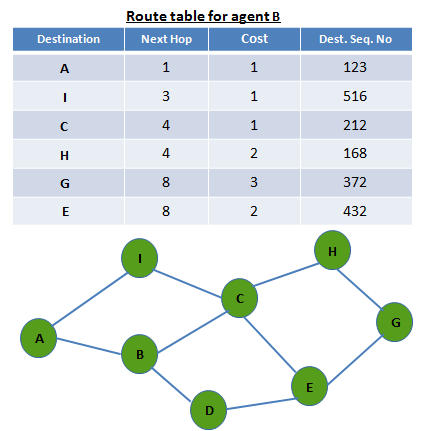
\includegraphics[scale = 0.75]{dest_seq}
\end{figure}

In the DSDV algorithm, each node transmits the updates in its own sequence number and routing table. In the network, when two routes to the same destination are received from two different neighbors, the algorithm executes the following rules;\newline
	- Choose the node with the larger destination sequence number \newline
	- If the sequence numbers are equal, then choose the route with minimum number of hops and update the route table.

In Figure \ref{dest_seq_ref}, node B has destination sequence numbers to each destination in its route table. These numbers are used to update the network with the rules defined above, in the case of link addition and link brakes defined in following sections.
\newpage	
\subsubsection{DSDV Link addition}

Figure \ref{linkk_addition} shows a sample link addition condition to the robot network. In this example, robot A joins the network by creating a radio link with robot B. When a new node A joins the network, it transmits of its own route table including the destination to itself $<A,A,0,101>$. Then the following procedure will be handled during iterations; \newline
	-Node B receives the the transmission of A and inserts a new line into its route table with $<A,A,1,101>$ and propagates this new node to its neighbors \newline
	-Node C and Node D receives this transmission and inserts the new route to their route tables with $<A,B,2,101>$

\begin{figure}[H]
\caption{An Example for Route Table} \label{linkk_addition}
\centering
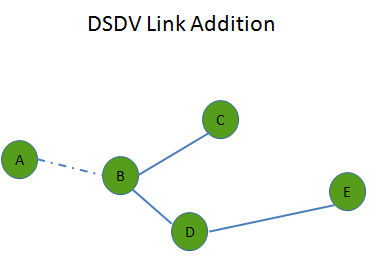
\includegraphics[scale = 0.65]{link_add}
\end{figure}	
		
\subsubsection{DSDV link breaks}

Figure \ref{linkk_brake} shows a sample link brake condition to the robot network. Robot B lost its connection with robot D. When the link between B and D breaks, node B gets no transmission from the D and notices the link breaks, then the following procedure will be handled; \newline
	- Node B update the cost for node D and E destinations to the infinity and increments the sequence numbers to these routes \newline
	- Node B propagates the updates to its neighbors and node A and node C updates the lines of the routes to the D and E, since the message from B includes higher sequence numbers for those routes.
		
\begin{figure}[H]
\caption{An Example for Route Table} \label{linkk_brake}
\centering
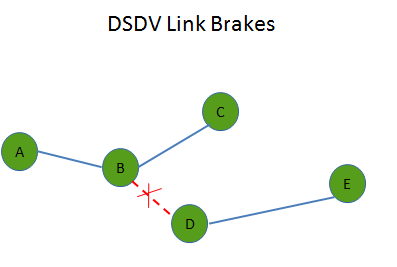
\includegraphics[scale = 0.65]{link_break}
\end{figure}
	
\subsection{Handling Lost Agents} \label{LostAgents}
The minimum number of position beacons required for the trilateration process is three for a two dimensional localization problem as illustrated in Section \ref{Trilateration_Process_ref} . Since the agents are assumed to have a narrow communication range, it is possible to not to find three  position beacons as direct neighbors for any agent at an instant time. In this case, it will not be possible to relocate these agents with trilateration and the position$\&$velocity data will drift from the real values with the increasing time passed without trilaterions. It is important to have a solution for this problem to keep the swarm together and to increase the robustness of the system against different environmental conditions. In our algorithm, concept of `Lost` agents and the procedures for these type of agents are described as follows:
	
	* An agent gets into 'Lost' mode, if it doesn't find at least three direct neighbors of position beacons at an instant time \newline
	* If an agent is in 'Lost' mode and missed the localization process for three times, it will get into 'Return to Home' mode \newline
	* If an agent is in 'Return to Home' mode, it will directly try to reach to the center of the desired formation shape.
		
The idea behind the 'Return to Home' mode is basically to increase the possibility of finding position beacons which are direct neighbors of the lost agent by directing it to the center of the swarm. A simple demonstration of this procedure is illustrated in Figure \ref{return_home_ref}
	
\begin{figure}[H]
\caption{Return to Home Approach of a Lost Agent} \label{return_home_ref}
\centering
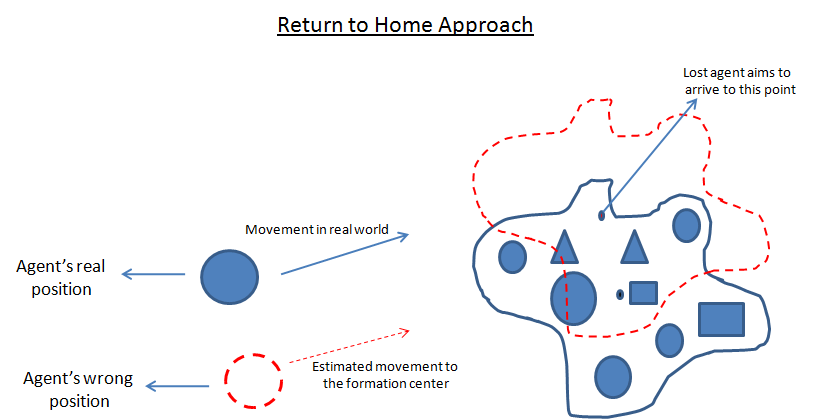
\includegraphics[scale = 0.60]{return_home}
\end{figure}
	
The lost agent aims to reach to the center of the formation and due to the errors on its position$\&$velocity data, it is expected to arrive to the red point illustrated in the figure. With this maneuver, the lost agent still have a chance to meet some position beacons in the swarm even if it directs itself to an incorrect goal state.
	
\subsection{State Estimation Procedure} \label{StateEstimationref}
In local positioning subsystem, second type agents are expected to execute a state estimator algorithm in which they propagate their state vectors composed of translational position and velocities with the help of inertial measurements. As discussed at the introduction of Section \ref{LOCAL POSITIONING SYSTEMS_ref} agents will update and correct their positions with the measurements provided by the trilateration process execeuted with the localization timer period. A Kalman estimator algorithm which uses the trilateration outputs as external measurements and the inertial measurements as inputs, is designed to fuse the inertial measurements with the trilateration calculations. The model for this observer system is defined as follows:
	
The state vector for each agent is defined as:

\begin{equation}
x_k = \begin{bmatrix}
X_k \\
\dot{X}_k\\
\end{bmatrix}
\end{equation}
	
where $X_k$ is the position and $\dot{X}_k$ is the velocity of the agents in x coordinates in two dimensional environment. All of the following procedures will be handled exactly the same for the state vector defined in y coordinates.

The discrete linear model is defined with the state equation of \cite{wiki_kalman}:

\begin{equation}
x_{k+1} = F_k     x_{k} + B_ku_k + w_k
\end{equation}
	
where $w_k$ is the process noise and 
\begin{equation}
F = \begin{bmatrix}
1 & d_t\\
0 & 1
\end{bmatrix}   
\end{equation}
	
\begin{equation}
B = \begin{bmatrix}
\frac{{d_t}^2}{2} \\
d_t
\end{bmatrix}
\end{equation}

where $d_t$ is the propagation period and $u_k$ is the translational acceleration measured with the help of inertial sensors. We add a random bias on the acceleration measurements on each agents acceleration input with maximum value of 0.1 mg \cite{bias}. Also, we add a white noise to the acceleration values with zero mean and 0.01 $[m/s^2]$ standart deviation \cite{noise}. The values of bias and noise terms are added to the measurements consistent with the specifications of industry grade inertial measurement units presented by the manufacturers.

The observation(external measurement) which will be calculated with the trilateration process :

\begin{equation}
z_k = H_kx_k + v_k
\end{equation}

where $v_k$ is the measurement noise. We add a noise component to this external measurement modeled with a Gaussian distribution with zero mean and 2$[m]$ standart deviation. This noise simulates the errors on the distance measurements handled with TOA methods. Since the trilateration process will provide new position data to the agents:
\begin{equation}
H_k = \begin{bmatrix}
1\\0
\end{bmatrix}
\end{equation}
	
The noise models for the process and the measurement are modelled with:

\begin{equation}
 w_k = \mathcal{N}(\mathbf{0,Q_k})
\end{equation}
	
\begin{equation}
v_k = \mathcal{N}(\mathbf{0,R_k})
\end{equation}
		
where $w_k$ is the process noise with zero mean multivariate normal distribution with covariance of $Q_k$ and $v_k$ is the measurement noise with zero mean Gaussian distribution with a variance of $R_k$
		
The filter has two main subsections named propagate and update phases. The update phase of the filter is executed after each trilateration process. The filter equations are as follows:
		
Propagation phase:

\begin{equation}
\hat{x}_{k,k-1} = F_k\hat{x}_{k-1,k-1} + B_ku_k
\end{equation}
		
\begin{equation}
 P_{k,k-1} = F_k P_{k-1,k-1}F^T_k + Q_k
\end{equation}
		
Update Phase:
\begin{equation}
\tilde{y}_k = z_k - H_k  \hat{x}_{k,k-1} 
\end{equation}

\begin{equation}
S_k = H_k P_{k,k-1} H^T_k + R_k
\end{equation}

\begin{equation}
K_k =  P_{k,k-1} H^T_kS_k^{-1}
\end{equation}
		
\begin{equation}
 \hat{x}_{k,k} =  \hat{x}_{k,k-1} + K_k \tilde{y}_k
\end{equation}
		
\begin{equation}
P_{k,k} = (I - K_kH_k)P_{k,k-1}
\end{equation}
		
where $Q_k$ is the process covariance matrix and $R_k$ is the measurement covariance. These variables are calculated as follows (by taking $\sigma_{acc} = 0.01[m/s^2]$ , $\sigma_{meas} = 2[m]$ and $d_t = 0.5 seconds$)

\begin{equation}
Q_k = \begin{bmatrix}
\sigma_{acc} * \frac{d^2_t}{2} & 0 \\
0 & \sigma_{acc} * d_t
\end{bmatrix}
\end{equation}
		
\begin{equation}
R_k = \sigma_{meas}
\end{equation}
		
In the above equations $K_k$ represents the Kalman gain matrix and $S_k$ is the residual covariance of the system at time $k$. $\hat{x}_{k,k}$ is the posteriori state estimate updated with measurements at time $k$ ;  $\hat{x}_{k,k-1}$ is the priori estimate of the state vector predicted with inputs at time $k$; $P_{k,k}$ is the posteriori error covariance matrix updated with measurements at time $k$; $P_{k,k-1}$ is the priori estimate covariance predicted with the inputs at time $k$.
			
\section{FORMATION CONTROL} \label{formation_control_ref}
The details of different methodologies for dynamical formation control with heterogeneous mobile robots is presented in this subsection. We have implemented three different approaches as Artificial Forces method, Bubble Packing method and Randomized Fractals method. It is possible to classify these methods in two sub categories. Potential field based approaches implements artificial forces acting on agents to get inside and cover the desired formation shape homogeneously by avoiding collisions between the agents. The resultant positions of the agents in the formation shape is not certain, it dynamically changes with the instantaneous positions and interactions of the agents with each other and environment. Two other methods , shape partitioning based approaches which are Bubble Packing and Randomized Fractals methods, share a common structural basis. In these approaches the complex formation shape is partitioned into goal states to cover the shape homogeneously with the mobile robots. The assignment of the agents to these goal states is handled with special algorithms to optimize the total displacements of the agents in the environment. The difference between these two methods is the partitioning approach of the formation shape. Figure \ref{formation_controlin_figi} illustrates different methodologies implemented in this project.
		
\begin{figure}[H]
\caption{Formation Control Topologies} \label{formation_controlin_figi}
\centering
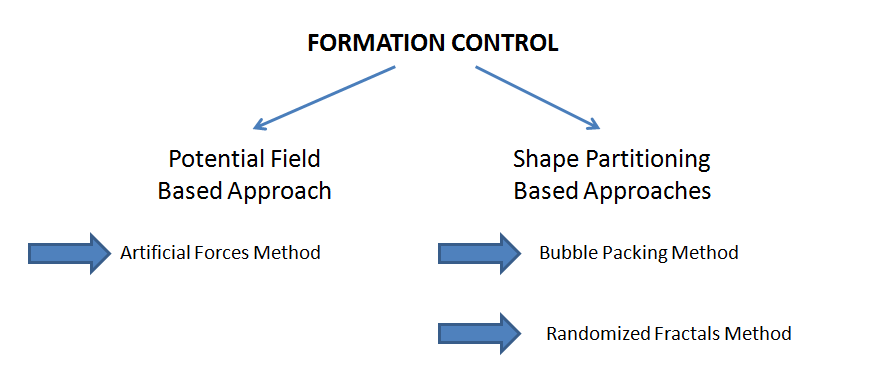
\includegraphics[scale = 0.60]{methods}
\end{figure}		
		
\subsection{Potential Field Based Approach}

\subsubsection{Artificial Forces Method} \label{Artificial Forces Ref} \label{Artificial_forces_ref}
In Artificial Forces method we have implemented potential fields over each agent arised from the interactions between agents, formation shape and environment. The positions of the agents at the formation shape  are determined with local equilibrium of the swarm in which every agent is at balance under the total force acting from the environment. There are basically three different kinds of artificial forces named; intermember forces representing the forces created by the other agents in the swarm to achieve collision avoidance, the attractive forces representing the forces created by the desired formation shape to attract the agent into the shape and repulsive forces created by the formation shape to keep agents inside the desired formation shape. It is possible to augment these type of forces for specific tasks and objectives. For example, obstacle forces created by the obstacles in the environment can be implemented to achieve obstacle avoidance. Since the method to calculate the artificial forces involves contour integrals, it will be useful to give mathematical definition of contour integrals.
		
Consider a curve $C$ which is a set of points $z = (x,y)$ in the complex plane defined by \cite{wiki_contour}

\begin{equation}
x = x(t),   \hspace{0.1cm} y = y(t),  \hspace{0.1cm} a\leq t \leq b
\end{equation}

where $x(t)$ and $y(t)$ are continuous functions of the real parameter $t$.  It is possible to write
		
\begin{equation}
z(t) = x(t)+iy(t),   \hspace{0.1cm} a\leq t \leq b
\end{equation}
		
This curve is called smooth if $z(t)$ has continuous derivative for all points along the curve, and it is called simple if it does not cross itself as defined in Equation \ref{crossitself}

\begin{equation} \label{crossitself}
z(t_1) \neq z(t_2)   \hspace{0.1cm} whenever   \hspace{0.3cm} t_1\neq t_2
\end{equation}
		
On the other hand if  $z(a)=z(b)$ is the only intersection point, the curve is said to be simple closed curve \cite{wiki_contour}. Regarding with these given definitions, an example for a  simple smooth closed curve is illustrated in Figure \ref{simple_closed_curve_ref}

\begin{figure}[H]
\caption{A Simple Closed Curve} \label{simple_closed_curve_ref}
\centering
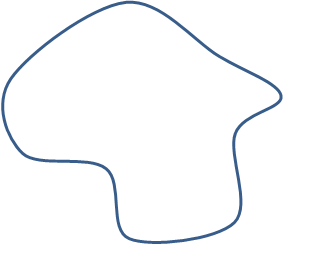
\includegraphics[scale = 0.60]{simple_closed_curve}
\end{figure}
		
Let $f(z)$ is a complex function in a domain $D$ in the complex plane and let $C$ be simple closed contour contained in $D$ with initial point $a$ and terminal point  $b$. It is possible to take the integral of $f(z)$ along the contour $C$ \cite{wiki_contour}
		
\begin{equation}
\oint_C f(z) dz = \int_{a}^{b} f(z(t))\frac{dz(t)}{dt} dt
\end{equation}
		
where
\begin{equation}
\frac{dz(t)}{dt} = \frac{dx(t)}{dt} + i\frac{dy(t)}{dt},   \hspace{0.1cm} a\leq t\leq b
\end{equation}
		
To simplify this equation, one can write $f(z) = u(x,y) + iv(x,y)$ and $dz = dx + idy$ into the statements,
		
\begin{align} \label{contour_integral}
\begin{split}
\oint_C f(z)dz & = \oint_C u dx - v dy + i \oint_C u dy + v dx \\
&= \int_{a}^{b}\left[u(x(t),y(t) )\frac{dx(t)}{dt} - v(x(t),y(t) )\frac{dy(t)}{dt}\right]dt\\
& \hspace{0.4cm} + i\int_{a}^{b} \left[u(x(t),y(t) )\frac{dy(t)}{dt} + v(x(t),y(t) )\frac{dx(t)}{dt}\right]dt
\end{split}
\end{align}

We have used this explicit form of the contour integrals in utility functions described in the following section. 		
		
\paragraph{Utility Functions}\hspace{0pt} \\
As it is mentioned in the Section \ref{Objectives}, the formation shapes will be simple closed contours which cannot be identified analytically. Definitions of the utility functions given in the following section are given with continuous contour integrals which requires the analytical expression of the curve on which the integral will be taken. In our thesis work, we have modified these expressions in discrete domain to provide a solution to  these type of calculations without analytical expressions of the closed curves.\\

\textit{ 		1- Cauchy Winding Number:} \\ 
Cauchy winding number of a curve in the plane around a given point is the number of times that curve travels counter-clockwise around the point. Suppose $C$ is the closed curve which is a set of points $z=(x,y)$ in the complex plane  and $z_i$ is a point to check whether it is inside of the curve or not, then the Cauchy winding number is \cite{17} :
					
\begin{equation}
 n(C,z_i) = \frac{1}{2\pi i}\oint_C \frac{dz}{z-z_i}
\end{equation}
		
The winding number for agent $i$ in the swarm,

\begin{equation}
n(C,z_i) = \left\{ \begin{array}{rl}
1 &\mbox{ when member i is inside C} \\
0 &\mbox{ when member i is outside C}
\end{array} \right.
\end{equation}

We have used this winding number to switch on/off some of the artificial forces while the agent is inside or outside of the formation shape. We have redefined this statement in discrete domain as:
\begin{equation}
n(C,z_i) = \frac{1}{2\pi i} \oint_C f(z)dz
\end{equation}

where 

\begin{equation}
f(z) = \frac{1}{z-z_i}
\end{equation}
		
Function of $f(z)$ can be partitioned into real and complex parts as:

\begin{equation}
u(x,y) = real(f(z))  \hspace{0.2cm} and \hspace{0.2cm} v(x,y) = imag(f(z))
\end{equation}
		
partitioning this function as mentioned in Equation \ref{contour_integral}
\begin{equation}
\oint_C f(z)dz  = \oint_C u dx - v dy + i \oint_C u dy + v dx 
\end{equation}

then

\begin{equation}
n(C,z_i)  = \frac{1}{2\pi i} \left[\int_{a}^{b} \left(u\frac{dx}{dt} - v\frac{dy}{dt}\right)dt + i\int_{a}^{b}\left(u\frac{dy}{dt} + v\frac{dx}{dt}\right)dt\right]
\end{equation}
		
Discrete contour integral representation of this equation is
		
\begin{equation}
n(C,z_i)  = \frac{1}{2\pi i} {\left[\sum_{k=1}^{K} {A_k} + i\sum_{k=1}^{K} {B_k}\right]}
\end{equation}

where
\begin{equation}
A_k = u(x_{k+1} - x_k ) - v(y_{k+1} -y_k )
\end{equation}

\begin{equation}
B_k = u(y_{k+1} - y_k ) + v(x_{k+1} - x_k)
\end{equation}


\begin{equation}
\norm{z_k - z_{k-1}} = \norm{z_{k+1} - z_k}, \hspace{0.2cm}  \forall k ;  \hspace{0.2cm} k=1,2,...,K \hspace{0.2cm} when  \hspace{0.2cm} K \to\infty
\end{equation}

The assumption of $K \to\infty$ makes it possible to calculate the integral of Cauchy winding number with a small error with large number of $K$ which can be achieved by partitioning the desired formation shape  into small pieces with equal $p2$ norms. We have used this approach to provide representations of the contour integrals in discrete domain. 

Figure \ref{iceride_disarida_refe} shows the test results for the grid map of an environment with a formation shape, where green dots represents the inner points of formation shape and red dots represents the outer points of the formation shape. Inner points in the grid map have a Cauchy winding number of 1, and the outer points have a Cauchy winding number of 0 .

\begin{figure}[H]
\centering
\captionsetup{format=hang,justification=centerfirst}
\caption{Formation Shape in an Environment} \label{iceride_disarida_refe}
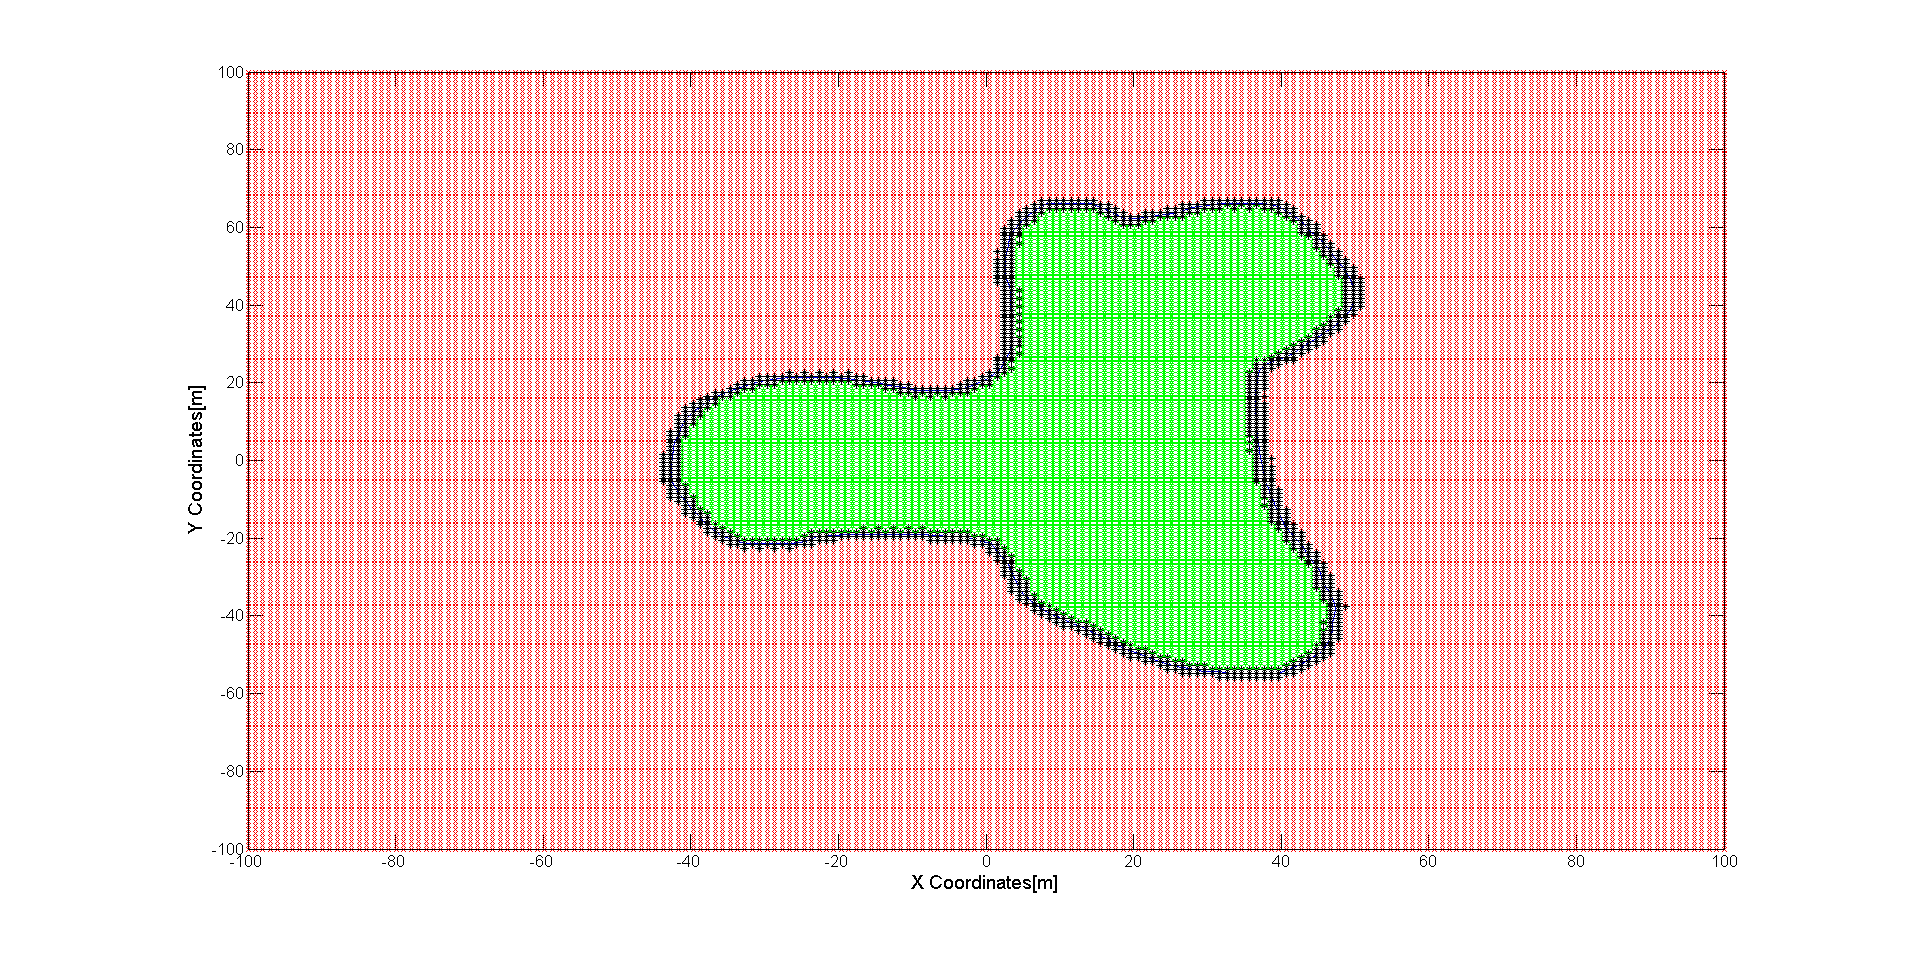
\includegraphics[scale = 0.28]{iceride_disarida}
\end{figure}

\textit{ 	2- Length of a formation shape} \\ 
The length of a formation shape can be calculated with the equation of \cite{17};
		
\begin{equation}
l(C)= \oint_C \norm{dz}
\end{equation}
		
We have redefined this expression for this contour integral with points of   $z_k = (x_k,y_k)$ in the complex plane

\begin{equation}
l(C) = \sum_{k=1}^{K}\sqrt{(x_{k+1} - x_k)^2 + (y_{k+1} - y_k)^2}
\end{equation}

where

\begin{equation}
\norm{z_k - z_{k-1}} = \norm{z_{k+1} - z_k}, \hspace{0.2cm}  \forall k ;  \hspace{0.2cm} k=1,2,...,K \hspace{0.2cm} when  \hspace{0.2cm} K \to\infty
\end{equation}
		
\textit{ 	3-Center of a Formation Shape} \\ 	
The center of a formation shape can be calculated with the equation of \cite{17};

\begin{equation} \label{center_formation_ref}
 z_c = \frac{\oint_C z\norm{dz}}{l(C)}
\end{equation}
		
We have redefined the discrete domain expression for Equation \ref{center_formation_ref} with points of  $z_k = (x_k,y_k)$ in the complex plane

\begin{align}
\begin{split}
&z_{cx} = \frac{\sum_{k=1}^{K}x(k)}{K}  \\
&z_{cy} = \frac{\sum_{k=1}^{K}y(k)}{K}  
\end{split}
\end{align}
		
where $z_{cx}$ and $z_{cy}$ are the $x$ and $y$ coordinates of the center of formation shape respectively and

\begin{equation}
\norm{z_k - z_{k-1}} = \norm{z_{k+1} - z_k}, \hspace{0.2cm}  \forall k ;  \hspace{0.2cm} k=1,2,...,K \hspace{0.2cm} when  \hspace{0.2cm} K \to\infty
\end{equation}

\textit{ 	4- Area of a Formation Shape} \\ 		
Green's theorem can be used to calculate the area of a closed curve. According to this theorem, the area of $D$ given by the double integral \cite{calculus}

\begin{equation}
 A = \int\int_D dA
\end{equation}
		
can be calculated with the line integral of

\begin{equation}
 A = \oint_D F ds = \frac{1}{2} \oint_D xdy - ydx
\end{equation}

where

\begin{equation}
F(x,y) = (-y/2,x/2)
\end{equation}
		
This contour integral can be reduced down to

\begin{align} \label{area_formation_ref}
\begin{split}
Area &= \frac{1}{2} \oint_C xdy - \frac{1}{2} \oint_C ydx \\
&= \frac{1}{2} \int_{t=a}^{b} x(t)\frac{dy(t)}{dt}dt - \frac{1}{2} \int_{t=a}^{b}y(t)\frac{dx(t)}{dt}dt
\end{split}
\end{align}
		
We have implemented the expression in Equation \ref{area_formation_ref} in discrete domain with points of  $z_k = (x_k,y_k)$ in the complex plane
			
\begin{equation}
Area = \frac{1}{2} \sum_{k=1}^{K} x_k(y_{k+1} - y_k) - \frac{1}{2} \sum_{k=1}^{K}y_k(x_{k+1} - x_k)
\end{equation}
			
where

\begin{equation}
\norm{z_k - z_{k-1}} = \norm{z_{k+1} - z_k}, \hspace{0.2cm}  \forall k ;  \hspace{0.2cm} k=1,2,...,K \hspace{0.2cm} when  \hspace{0.2cm} K \to\infty
\end{equation}

\paragraph{Artificial Forces}\hspace{0pt} \\ 
Artificial forces are defined to gather the agents inside a formation shape and make them distributed homogeneously in the shape. It is possible to define some additional artificial forces to implement features like obstacle$\&$collision avoidance or smooth transitions between the boundaries of the formation shape. We have implemented attractive forces, repulsive forces, intermember forces, obstacle forces and transition forces to generate individual control laws for all agents in the swarm. Summation of these different types of artificial force components define the individual control law of a single agent. Suppose the state of a member $i$ is described by

\begin{equation}
X_i = \begin{bmatrix}
z_i\\ \dot{z}_i
\end{bmatrix}
\end{equation}

where  $z_i \in C$, represents the position of the $i^{th}$ member of the swarm. The state of the whole swarm $x= \begin{bmatrix}
X_1 & X_2 & ... X_n
\end{bmatrix}$ is determined by the linear equations of \cite{17}

\begin{equation}
\dot{x} = Ax + Bu
\end{equation}

where

\begin{align}
\begin{split}
&A = diag\left(\hat{A}\right)_{nxn}\\
&B = \frac{1}{m} diag\left(\hat{B}\right)_{nxn}
\end{split}
\end{align}

with

\begin{equation}
\hat{A} = \begin{bmatrix}
0&1\\0&0
\end{bmatrix} , \hspace{0.2cm} \hat{B} = \begin{bmatrix}
0&1
\end{bmatrix}
\end{equation}
			
The vector for individual control laws of the swarm

\begin{equation}
u = \begin{bmatrix}
u_1 & u_2 & ... & u_n
\end{bmatrix}
\end{equation}

where

\begin{equation}
u_i = F_{i,a} + F_{i,r} + F_{i,m} + F_{i,t}
\end{equation}

We have defined the concept of "coverage circle"	for the agents which will be used in the artificial forces calculations. Coverage circle of agent $i$, $C_i$, is defined as the circle with minimum radius which can cover the whole agent's collision surface. The radius of this circle is given with $d_c$. Some of the examples of coverage circles for different types of mobile robots are illustrated in Figure \ref{coverage_circle_ref} below
		
\begin{figure}[H]
\caption{Coverage Circles of Different Types of Agents} \label{coverage_circle_ref}
\centering
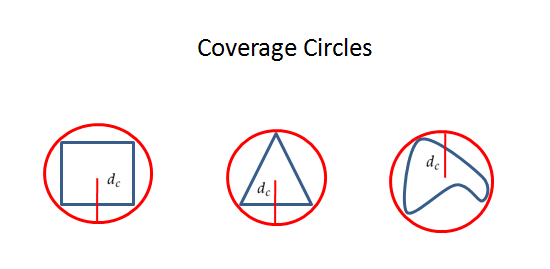
\includegraphics[scale = 0.60]{coverage_circles}
\end{figure}
		
Different artificial force components are described in details at the following section. \newline

\textit{			1- Attractive Forces} \\ 
Attractive forces are the artificial force components generated by the formation shape to attract the agent towards the center of the formation .They are active when the agents are outside of the shape. 

\begin{figure}[H]
\caption{Attractive Forces Generated by the Formation Shape}
\centering
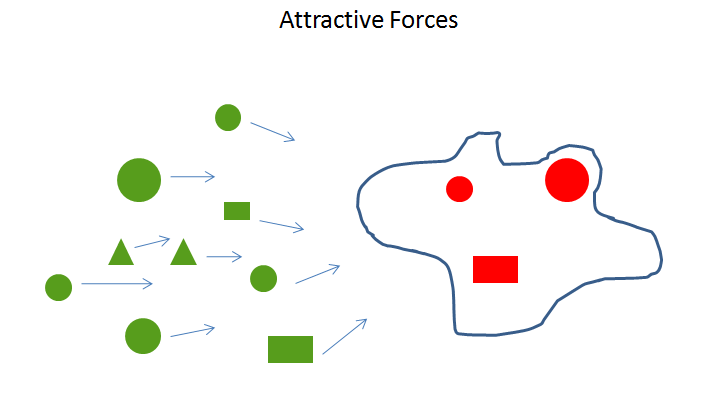
\includegraphics[scale = 0.60]{attractive_forces}
\end{figure}	

The equations for the attractive forces are defined as follows in \cite{17}:			

\begin{equation} \label{samitha_attractive}
F_{i,a} := \frac{k_a (1-n(C,\alpha X_i))}{l(C)} \oint_C(z-\alpha X_i)\norm{dz}
\end{equation}

where $k_a$ is the variable gain and $\alpha = \begin{bmatrix}
1 & 0
		\end{bmatrix}$. Equation \ref{samitha_attractive} takes the contour integral of the curve defined by desired formation shape. Since we don't have the analytical expression of the desired formation shape, we have redefined this expression in discrete domain. The representation of the attractive forces on agent $i$ on $z_i = (x_i, y_i)$ with the points of  $z_k = (x_k,y_k)$ of formation shape in the complex plane \cite{17}:

\begin{align}
\begin{split}
& F_{iax} =\frac{k_a (1-n(C,\alpha X_i))}{l(C)}  \sum_{k=1}^{K} (x_k  - x_i)\\
& F_{iay} =\frac{k_a (1-n(C,\alpha X_i))}{l(C)}  \sum_{k=1}^{K} (y_k  - y_i)\\
\end{split}
\end{align}
			
where

\begin{equation}
\norm{z_k - z_{k-1}} = \norm{z_{k+1} - z_k}, \hspace{0.2cm}  \forall k ;  \hspace{0.2cm} k=1,2,...,K \hspace{0.2cm} when  \hspace{0.2cm} K \to\infty
\end{equation}
			
and $F_{iax} , F_{iay} $ are the attractive force components in $x,y$ coordinates respectively.\newline
			
\textit{	2- Repulsive Forces} \\ 
Repulsive forces are the artificial force components generated by the formation shape to keep the agents inside the shape. They are active when the agents are inside the shape. 
					
\begin{figure}[H]
\caption{Repulsive Forces Generated by the Formation Shape}
\centering
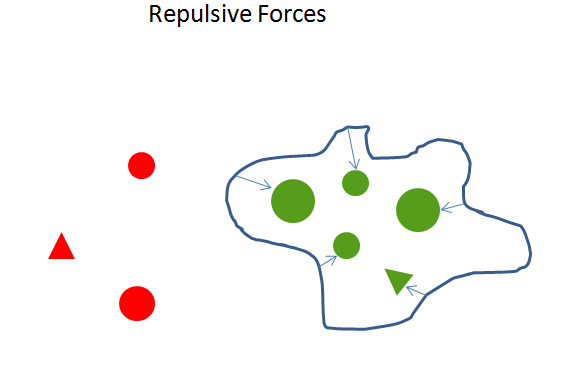
\includegraphics[scale = 0.60]{repulsive_forces}
\end{figure}
							
The equations for the repulsive forces are defined as follows \cite{17}:	

\begin{equation} \label{samitha_repulsive}
F_{i,r} := k_r  n(C,\alpha X_i) \oint_C \left[\frac{\alpha X_i - z}{\norm{\alpha X_i - z}^3}\right] \norm{dz}
\end{equation}

where $k_r$ is the variable gain for the repulsive forces. We have redefined the Equation \ref{samitha_repulsive} in discrete domain to calculate the repulsive forces for complex shapes. The representation of the repulsive forces on agent $i$ on $z_i = (x_i, y_i)$ with the points of  $z_k = (x_k,y_k)$ of formation shape in the complex plane:

\begin{align}
\begin{split}
& F_{irx} = k_r n(C,\alpha X_i)  \sum_{k=1}^{K} \frac{x_i - x_k}{\norm{\alpha X_i - z_k}^3}\\
& F_{iry} = k_r n(C,\alpha X_i)  \sum_{k=1}^{K} \frac{y_i - y_k}{\norm{\alpha X_i - z_k}^3}
\end{split}
\end{align}
				
where

\begin{equation}
\norm{z_k - z_{k-1}} = \norm{z_{k+1} - z_k}, \hspace{0.2cm}  \forall k ;  \hspace{0.2cm} k=1,2,...,K \hspace{0.2cm} when  \hspace{0.2cm} K \to\infty
\end{equation}
						
and $F_{irx} , F_{iry} $ are the repulsive force components in $x,y$ coordinates respectively. \newline
						
\textit{		3- Inter-member repulsion forces} \\ 
Intermember forces are the artificial force components generated by the agents in the swarm to avoid collisions between themselves. 
			
\begin{figure}[H]
\caption{Intermember Forces Generated by Agents}
\centering
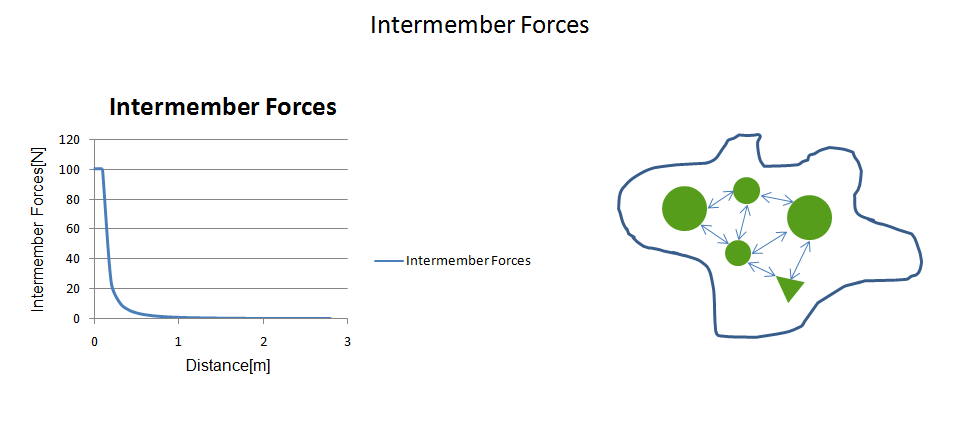
\includegraphics[scale = 0.60]{intermember_forces}
\end{figure}
			
The equations for the intermember forces on the agent $i$ on $z_i = (x_i, y_i)$  in the complex plane \cite{17},
			
\begin{equation}
F_{i,m} = k_m \sum_{j=1, j\neq i}^{N}\frac{\alpha X_i - \alpha X_j}{(\norm{\alpha X_i - \alpha X_j})} \frac{1}{(\norm{\alpha X_i - \alpha X_j} - d_o)^2}
\end{equation}
			
where $d_o$ is the total distance between the center of coverage circles of agents which can be calculated with

\begin{equation}
 d_o = d_{c_i} + d_{c_j}
\end{equation}			

The force components in x,y coordinates respectively,

\begin{align}
\begin{split}
&F_{imx} = k_m \sum_{j=1, j\neq i}^{N}\frac{x_i- x_j}{\norm{\alpha X_i - \alpha X_j}}  \frac{1}{(\norm{\alpha X_i - \alpha X_j} - d_o)^2}\\
&F_{imy} = k_m \sum_{j=1, j\neq i}^{N}\frac{y_i- y_j}{\norm{\alpha X_i - \alpha X_j}}  \frac{1}{(\norm{\alpha X_i - \alpha X_j} - d_o)^2}\\
\end{split}
\end{align}
		
where $k_m$ is the variable gain for the intermember forces.  \newline
			
\textit{4- Transition Forces} \\ 		
Transition forces are the artificial force components to force the agent to get inside the formation shape when they are close to the boundaries. Since the attractive forces have a decreasing nature while the agent getting closer to the formation shape, we need to add this type of forcing function to ensure the agents to get inside the shape. Transition forces are active outside of the desired formation shape.
			
\begin{figure}[H]
\caption{Comparison of Attractive and Transition Forces}
\centering
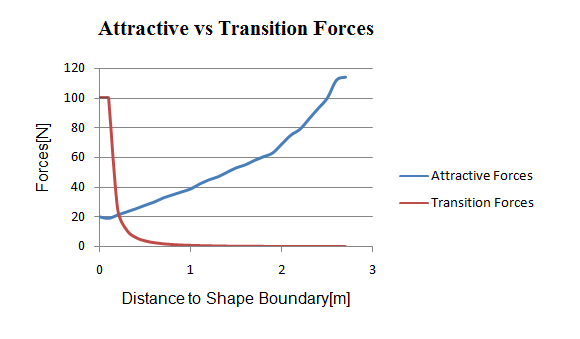
\includegraphics[scale = 0.80]{transition_forces}
\end{figure}		

The equation for the transition forces are defined as follows \cite{17}:	
				
\begin{equation}
F_{i,t} = k_t (1-n(C,\alpha X_i) \oint_C \frac{z-\alpha X_i}{\norm{z-\alpha X_i}}\norm{dz}
\end{equation}
				
where $k_t$ is the variable gain for the transition forces. The representation of the transition forces on agent $i$ on $z_i = (x_i, y_i)$ with the points of  $z_k = (x_k,y_k)$ of formation shape in the complex plane:
			
\begin{align}
\begin{split}
&F_{itx} = k_t  (1-n(C,\alpha X_i) \sum_{k=1,}^{K}\frac{x_k- x_i}{\norm{\alpha X_i - z_k}^3}\\
&F_{ity} = k_t  (1-n(C,\alpha X_i) \sum_{k=1,}^{K}\frac{y_k- y_i}{\norm{\alpha X_i - z_k}^3}\\
\end{split}
\end{align}
			
where  $F_{itx} , F_{ity} $ are the transition force components in $x,y$ coordinates respectively and

\begin{equation}
\norm{z_k - z_{k-1}} = \norm{z_{k+1} - z_k}, \hspace{0.2cm}  \forall k ;  \hspace{0.2cm} k=1,2,...,K \hspace{0.2cm} when  \hspace{0.2cm} K \to\infty
\end{equation}					
			
\textit{			5- Obstacle forces} \\ 
Obstacle forces are the artificial force components generated by the obstacles in the environment to achieve obstacle avoidance of the agents during formation control. 	
The equation for the obstacle forces are defined as follows \cite{17}:	
			
\begin{equation} \label{samitha_obstacle}
F_{i,o} := k_o  \oint_O \left[\frac{\alpha X_i - z_o}{(\norm{\alpha X_i - z_o} - d_{c_i})^4}\right] \norm{dz_o}
\end{equation}
			
where $k_o$ is the variable gain for the transition forces and $d_{c_i}$ is the radius of coverage circle of agent $i$ . This contour integral is taken on the curve of the obstacle with  points of $z_o = (x_o,y_o)$ in the complex plane. Obstacles in the workspace are assumed to have complex shapes without mathematical definitions. We have expressed the Equation \ref{samitha_obstacle} in discrete domain. The representation of the obstacle forces on agent $i$ on $z_i = (x_i, y_i)$ with the points of  $z_{ok} = (x_{ok},y_{ok})$ of formation shape in the complex plane:
			
\begin{align}
\begin{split}
& F_{iox} = k_o   \sum_{k=1}^{K} \frac{x_i -x_{ok}}{(\norm{\alpha X_i - z_{ok}} -d_{c_i})^4}\\
& F_{ioy} = k_o   \sum_{k=1}^{K} \frac{y_i - y_{ok}}{(\norm{\alpha X_i - z_{ok}} -d_{c_i})^4}\\
\end{split}
\end{align}
			
where

\begin{equation}
\norm{z_k - z_{k-1}} = \norm{z_{k+1} - z_k}, \hspace{0.2cm}  \forall k ;  \hspace{0.2cm} k=1,2,...,K \hspace{0.2cm} when  \hspace{0.2cm} K \to\infty					
\end{equation}
			
\paragraph{Buffer Zone Implementation}\hspace{0pt} \\
The attractive and transition forces are defined to be active when the agents are outside of the shape. On the other hand, the repulsive forces are active when agents are inside the shape. Because of the sharp transitions on the total artificial force acting on an agent which is crossing the boundary of the formation shape, it is possible to have a chattering effect. To avoid this chattering effect and provide a smooth transition of the agent to pass the boundary of formation shape, we have implemented a buffer zone defined around the boundaries of the formation shape. The main approach during the transition on the boundaries is to dynamically change the variable gains of these artificial forces linearly between zero and nominal values at the boundary conditions. The variable gains of the attractive and transition force components have their nominal values at the outer boundary of shape and these gains are decreased down to zero linearly while travelling towards the inner boundary of the shape. On the other hand, the variable gain for the repulsive forces has its nominal value at the inner boundary of the shape and this gain is decreased down to zero linearly while travelling towards to outer boundary of the shape.
     
\begin{figure}[H]
\caption{Transition of the Artificial Forces on Buffer Zone}
\centering
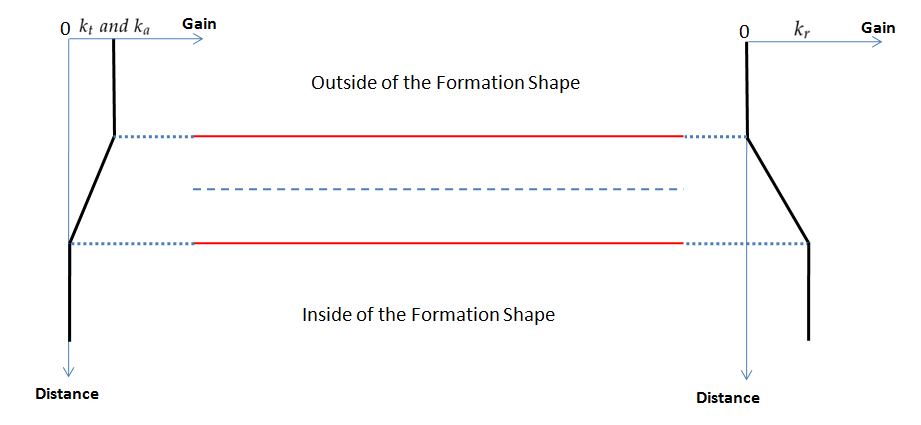
\includegraphics[scale = 0.50]{buffer_zone}
\end{figure}
					
\subsection{Shape Partitioning Methods} \label{shapepartition_ref}
In shape partitioning methods we have reduced down the formation control problem into two subproblems. The first part of the solution is to partition the desired formation shape into potential goal states according to the agent types to cover the desired formation shape homogeneously. We have proposed two different solutions to the shape partitioning problem in this thesis work, Bubble Packing method and Randomized Fractals method. The second part of the solution is the decision process to assign the agents to these goal states continuously to minimize the total displacement of swarm while achieving the desired formation shape. During this decision process, the cost of reaching different goal states is defined with the displacement on the shortest path while reaching that goal state. Our algorithm tries to reduce down these cost valus to minimize the total displacement of the swarm.

Shape partitioning methods have an approach to direct the agents to the goal states in which they have assigned dynamically. In this approach it is still needed to have collision avoidance algorithms to prevent the agents to collide with each other and workspace obstacles while travelling towards these goal states. For this purpose we add obstacle and inter-member forces to the individual control laws defined in shape partitioning approaches.
			
\subsubsection{Determining the Potential Goal States} \label{Partitioning_ref}
\paragraph{Bubble Packing Method} \hspace{0pt} \\				
Bubble Packing method is widely used in mesh generation problems. It basically depends on covering a curve, surface or a volume with a proper number of bubbles by packing them tightly which mimic a Voronoi diagram, from which a set of well-shaped Delaunay triangles can be created by connecting the centers of the bubbles \cite{27}.  The algorithm places the bubbles with their initial conditions in the environment and apply them interbubble forces which imitates the Van der Waals forces between the molecular bonds  to distribute the bubbles homogeneously. Here, the main idea is to generate a mesh for a surface with identical bubbles to mimic a regular Voronoi diagram with the vertices represented by the centers of these bubbles. On the other hand, adaptive population control  methods are developed to increase the number of bubbles to fill the gaps in the shape and to remove the excess bubbles which are overlapping with each other and the shape boundaries \cite{27}. 

Since the numbers and the the radius of coverage circles defined at Section \ref{Artificial Forces Ref} are predetermined in our formation control problem, the general bubble meshing algorithm have to be adapted to meet the requirements for shape partitioning in formation control.  In our project we have adapted this algorithm to represent the agents in the swarm as bubbles with the radius of their coverage circles and create a mesh by using these bubbles. The details of the implementation are given in following sections.\newline
			
\textit{			I - Initial Placements of the Bubbles} \\ 
The initial bubble placements are important because it will greatly reduce the convergence time of the partitioning process. In this work, we have initiated the bubbles close to the center of the formation shape randomly. The implemented algorithm for initial bubble placements is provided as follows:
			
\begin{algorithm}[H]
\KwData{Set of Bubbles, Desired Formation Shape }
\KwResult{Initial Placements of the Bubbles }
Initialize free configuration space $C_{free}$ as the desired formation shape \newline
\For{<Each Bubble $i$>}
{		
*Calculate the free configuration space,$C_{free}$, for bubble $i$\;
*Put the Bubble $i$ to the closest point to  formation center  $z_c$  in the free configuration space\;
*Add the agent $i$ into the configuration space as an obstacle \;
}\		
\caption{INITIALIZE$\_$BUBBLE$\_$POSITIONS} \label{intial_buble}
\end{algorithm}
		
The term free configuration space $C_{free}$ will be analyzed in detail in Section \ref{DecisionProcess Ref}. A simulation output, with a sample formation shape and 11 coverage circles which are representing a heterogeneous swarm composed of agents from 3 different size is illustrated in Figure \ref{algorithm1_ref} below.
		
\begin{figure}[H]
\caption{Initialization of the Bubble Packing Algorithm} \label{algorithm1_ref}
\centering
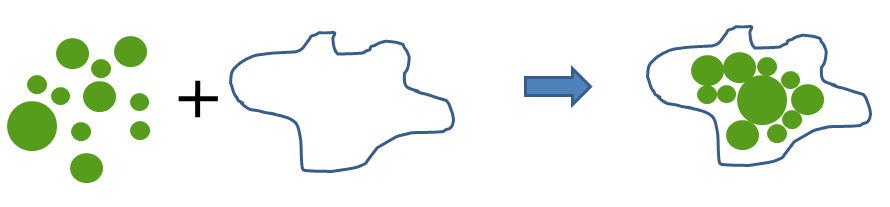
\includegraphics[scale = 0.50]{bubble_packing}
\end{figure}
				
\textit{			II- Bubble Meshing Process } \\ 
The bubbles are distributed homogeneously with this process under two kinds of forces, interbubble forces and shape repulsive forces. The interbubble forces are proximity-based forces so that a system of bubbles is in equilibrium when bubbles are distributed over the whole formation shape. The implemented force equation is given
		
\begin{equation}
f_i(l) = \left\{ \begin{array}{rl}
al^3 + bl^2 + cl + d &\mbox{ when 0 $\leq$ l $\leq$ $l_0$} \\
0                               &\mbox{ l > $l_0$}
\end{array} \right.
\end{equation}

where $l$ is the distance between the centers of the related bubbles and $a,b,c,d$ and $l_0$ are the variables to tune the force acting on the bubbles. 

\begin{figure}[H]
\caption{Interbubble Forces}
\centering
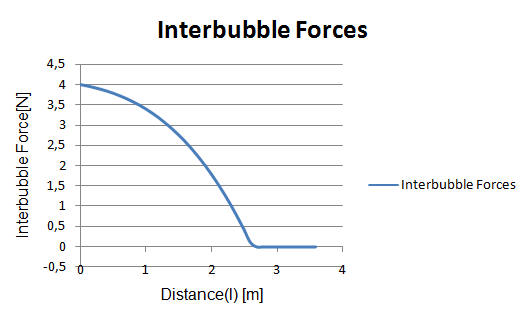
\includegraphics[scale = 0.70]{interbubble_forces}
\end{figure}
	
The shape repulsive forces have the same characteristics with the repulsive artificial forces discussed in Section \ref{Artificial Forces Ref}. The representation of shape repulsive forces for the desired formation shape $C$ with the points of  $z_k = (x_k,y_k)$ the complex plane:
	
\begin{equation} \label{buble_repulsive}
f_r(X_i) := \oint_C \left[\frac{\alpha X_i - z}{\norm{\alpha X_i - z}^3}\right] \norm{dz}
\end{equation}

where $k_r$ is the variable gain for the shape repulsive forces. We have defined the shape repulsive forces on agent $i$ in discrete domain with the points of  $z_k = (x_k,y_k)$ on formation shape in the complex plane:

\begin{equation}
f_r(X_i) = \sum_{k=1}^{K} \frac{\alpha X_i - Z_k}{\norm{\alpha X_i - z_k}^3}
\end{equation}
				
where

\begin{equation}
\norm{z_k - z_{k-1}} = \norm{z_{k+1} - z_k}, \hspace{0.2cm}  \forall k ;  \hspace{0.2cm} k=1,2,...,K \hspace{0.2cm} when  \hspace{0.2cm} K \to\infty					
\end{equation}
						

	
The bubbles are distributed homogeneously under the influence of these two forces and they get an equilibrium state in which the total net forces acting on individual bubbles reaches zero. Figure \ref{buble_ornek} shows a simulation output of Bubble Packing algoithm which is initialized with coverage circles derived from the output of the INITIALIZE$\_$BUBBLE$\_$POSITIONS algorithm. The coverage circles are homogeneously distributed in the formation shape with the help of inter-bubble and shape repulsive forces. The final equilibrium states of the bubbles determine the potential goal states $g_i \in G$  of the agents in the swarm to cover the formation shape.

\begin{figure}[H]
\caption{Bubble Packing Algorithm} \label{buble_ornek}
\centering
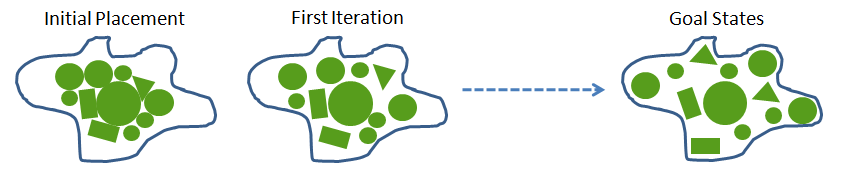
\includegraphics[scale = 0.62]{bubble_packing2}
\end{figure}

\paragraph{Randomized Fractals Method}\hspace{0pt} \\
Randomized fractals methods are used to cover surfaces or volumes randomly with fractals. The main idea is to fill the shapes iteratively with fractals which has the areas determined by the rule of \cite{26} :

\begin{equation} \label{fractals}
A_i = \frac{A}{\zeta(c,N)(i+N)^c}
\end{equation}

where $A$ is the total area to cover and $A_i$ is the area of the $i^{th}$ fractal. The parameters of $c$ and $N$ can be chosen to implement different changes on the fractals' areas with the increasing number of iterations with $c>1$ and $N>0$. Here  $\zeta$ is the Hurwitz function defined by

\begin{equation}
\zeta(c,N) = \sum_{i=0}^{\infty} \frac{1}{(i+N)^c}
\end{equation}

It is possible to write, 
	
\begin{equation}
\sum_{i=0}^{\infty}A_i = \sum_{i = 0}^{\infty}\left(\frac{A}{\zeta(c,N)(i+N)^c}\right)
\end{equation}
	
which tells us the sum of the all areas $A_i$ is the total area of $A$ and the algorithm is space filling. This approach implements the fractals infinitely by reducing the areas in accordance with the Equation \ref{fractals}, to cover the desired formation shape randomly. 

\begin{figure}[H]
\caption{Randomized Fractals \cite{26}}
\centering
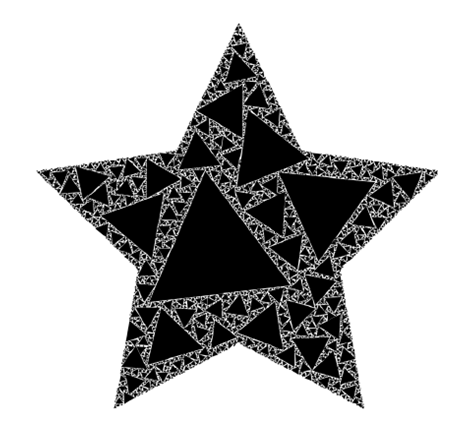
\includegraphics[scale = 0.60]{randomized}
\end{figure}
	
Types and the number of the agents, which will be represented with their coverage circles, are predetermined in our work. By using this constraint, we have adapted the randomized fractals algorithm as follows:
		
\begin{algorithm}[H]
\KwData{Set of Coverage Circles, Desired Formation Shape }
\KwResult{Potential Goal States }
Initialize free configuration space $C_{free}$ as the desired formation shape \newline
\For{<Each Coverage Circle $i$>}
{		
*Calculate the free configuration space $C_{free}$ for circle $i$\;
\eIf{$C_{free}  \neq Full$}{
*Put the circle $i$ randomly in $C_{free}$ \;
*Add the agent $i$ into configuration space as an obstacle \;
}{
*Break and warn the operator to increase the size of formation shape
}
}\												
\caption{RANDOMIZED$\_$FRACTALS$\_$ALGORITHM} 
\end{algorithm}
		
The algorithm iteratively checks the free configuration space that if there is enough space. If so, it inserts a coverage circle which is representing the current agent in the swarm, randomly in the desired formation shape. At the end of each insertion, it updates the free configuration space and jumps to next iteration. When algorithm terminates, the positions of the coverage circles which are randomly placed in desired formation shape gives us the goal states $g_i \in G$  of the agents. 

\begin{figure}[H]
\caption{Simulation Output of the Algorithm} \label{randomized_ornek}
\centering
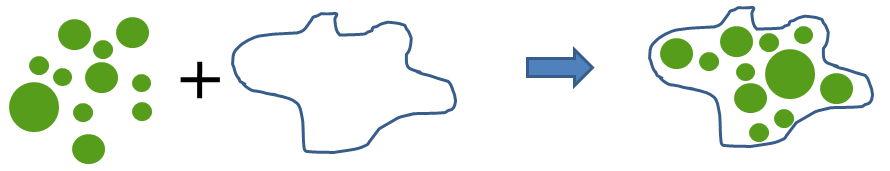
\includegraphics[scale = 0.60]{randomized_ornek}
\end{figure}

Figure \ref{randomized_ornek} shows a simulation output of the Randomized Fractals algorithm. In this figure, coverage circles are representing the members of a swarm which consist of 11 heterogeneous agents from 3 different sizes. These coverage circles are randomly distributed in the desired formation shape with the help of Randomized Fractals algorithm. Positions of the coverage circles define the goal states $g_i \in G$  of the agents in the formation shape. 

	
\subsubsection{Decision Process on Goal States}\hspace{0pt} \label{DecisionProcess Ref} \\
In Section \ref{Partitioning_ref}, we have reduced down the formation control problem in which every agent is expected to decide where to position in a given set of possible goal states $g_i \in G$ .  During this decision process, the cost of reaching different goal states will be the main criteria for each agent. Given goal states and cost values to these goal states, each agent must decide where to position in the formation. This process must be held to optimize the utility of every agent with a collaboration. It is obvious that some of the agents may want to choose the same goal point to reach, so the swarm must reach a global consensus on target points and cases including conflictions must be handled. Our main approach to provide a solution for this problem is to make each agent to calculate the costs of its own to reach the goal states $g_i \in G$ and then reach a global consensus with the other agents to minimize the overall displacements of the swarm. 

The algorithm which handles the assignment process of the agents to the goal states, is implemented in four stages. At the first stage, each agent calculates its own free configuration space. Secondly, agents calculate their visibility graphs by using their free configuration space. At the third stage,  agents calculate and report their costs to reach each of the goal states $g_i \in G$ with the help of Dijkstra's algorithm. These cost values are defined as the displacement to reach a goal state on shortest path.  Finally, agents are assigned to the goal states with the help of Hungarian algorithm which uses the cost values reported by the agents. Hungarian algorithm handles the assignment process to minimize the overall cost(i.e. total displacement) of the swarm.
	
\paragraph{Free Configuration Space}\hspace{0pt} \\
We have defined the shortest paths to the goal states of $g_i \in G$ in the free configuration space to avoid collisions with the workspace obstacles \cite{92}. In our implementation, each agent calculates its free configuration space by extracting the forbidden space from the configuration space itself. Forbidden space is calculated by augmenting the workspace obstacles with the help of Minkowski sums and we have implemented this process as follows.

Assume an environment with set of obstacles $S = \begin{Bmatrix}
P_1, P_2, .. P_t \end{Bmatrix}$. Configuration for agent $i$ can be described with the position of the center of its coverage circle with $R=\begin{Bmatrix}x_i, y_i\end{Bmatrix}$. Configuration space of $i^{th}$ agent is the workspace itself and represented by $C(R_i)$. This configuration space is composed of two subspaces; free configuration space and forbidden configuration space of agent $i$ \cite{92}.

\begin{equation}
C(R_i) = C_{free}(R_i,S) + C_{forb}(R_i,S)
\end{equation}

In our implementation each agent calculates its forbidden space by augmenting the workspace obstacles with the help of Minkowski sum method. Minkowski sum method is implemented as follows:

Let a single obstacle is described with a point set of $S_1$ and the agent is described with a point set of $S_2$. The Minkowski sum of these two sets $S_1 \subset R^2$ and $S_2 \subset R^2$ can be calculated with the following \cite{92},
	
\begin{equation}
S_1 \oplus S_2 := \begin{Bmatrix}
p+q : p \subset S_1, q \subset S_2
\end{Bmatrix} 
\end{equation}

where $p+q$ denotes the vector sum of the vectors $p$ and $q$.
		
\begin{figure}[H]
\caption{Forbidden Space Caused by an Obstacle \cite{92}} \label{yasakli_bolge}
\centering
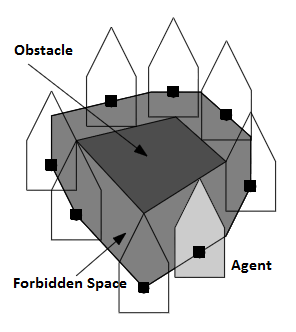
\includegraphics[scale = 0.75]{Forbidden}
\end{figure}
	
Figure \ref{yasakli_bolge} shows a forbidden space related with an obstacle. Forbidden space for agent $i$, $C_{forb}(R_i, S)$, is the sum of the forbidden spaces calculated for each obstacle in the environment \cite{92}. Agents extract their forbidden space $C_{forb}(R_i, S)$ from the configuration space itself to calculate their free configuration spaces.
	
\paragraph{Visibility Graphs and Dijkstra$'$s Algorithm}\hspace{0pt} \\
We have provided collision avoidance while travelling towards to the goal states $g_i \in G$ by defining the shortest paths in the free configuration spaces of the agents. In \cite{92}, an additional constraint for the shortest path is defined as follows : 

\begin{displayquote}
The shortest path between $p_{start}$ and $p_{goal}$ among a set $S$ of augmented polygonal obstacles consists of the arcs of the visibility graph $\gamma_{vis}(S^*)$ where $S^* := S \cup \begin{Bmatrix}
p_{start}, p_{goal}
\end{Bmatrix}$
\end{displayquote}

A visibility graph, $\gamma_{vis}(S^*)$, is a graph which is set of interior nodes representing the vertices of the set of obstacles, $S$, in the environment and edges which represents visible (which are not crossing and interior region of an obstacle) connections between these nodes \cite{92}.

In this project we have updated this constraint in our algorithm. We have inserted all of the goal states $g_i \in G$ in the visibility graphs of each agent to calculate the shortest paths to all of these goal states rather than a specific $p_{start}$ and $p_{goal}$ points given in the definition. In the implementation phase, we have used the obstacles which are augmented with the Minkowski sums to calculate the free configuration space. Let these set of augmented polygonal obstacles represented with $S_i \subset S$. 



Algorithm to calculate the visibility graph of  $S^* := S \cup \begin{Bmatrix}
g_i \in G
\end{Bmatrix}$
	
\begin{algorithm}[H]
\KwData{Set of Vertices Included in $S^*$ }
\KwResult{Visibility Graph of $S^*$ }
Initialize a graph $\gamma = (V,E)$ where $V$ is the set of al vertices of the polygons in $S^*$ and $E = \oslash$  \\
\For{<all vertices $v \subset V$>}
{		
W = VISIBLE$\_$VERTICES($v$,S)\;
Add edges W to list E\;
}\

\caption{VISIBILITY$\_$GRAPH}
\end{algorithm}

where $VISIBLE$\_$VERTICES(v,S)$ algorithm checks whether line segments drawn from $v$ to all vertices in $S$ is intersecting an interior area of any obstacle in the environment and returns the non-intersecting edges.  With the help of this $VISIBILITY$\_$GRAPH$ algorithm $SHORTEST$\_$PATH$ algorithm can be defined as follows. \newline
	
\begin{algorithm}[H]
\KwData{A set $S$ of disjoint polygonal obstacles, position of agent, $p_{start}$, and all goal states $g_i \in G$}
\KwResult{The shortest collision-free paths from $p_{start}$ to all goal states $g_i \in G$}
* Assign $\gamma$ = VISIBILITY$\_$GRAPH$(S^*)$ \newline
* Assign each arc $(v,w)$ in $\gamma_{vis}$ a weight, which is the Euclidian length of segment $vw$ \newline
\For{<Each goal state $g_i \in G$>}
{
* Use Dijkstra's algorithm to compute a shortest path between $p_{start}$ and $g_i \in G$ in $\gamma_{vis}$
}
\caption{SHORTEST$\_$PATH}
\end{algorithm}
  
\vspace{2cm}

\begin{figure}[H]
\caption{Shorthest Paths to Goal States $g_i \in G$ in a Visibility Graph} \label{dijksttae_visibility}
\centering
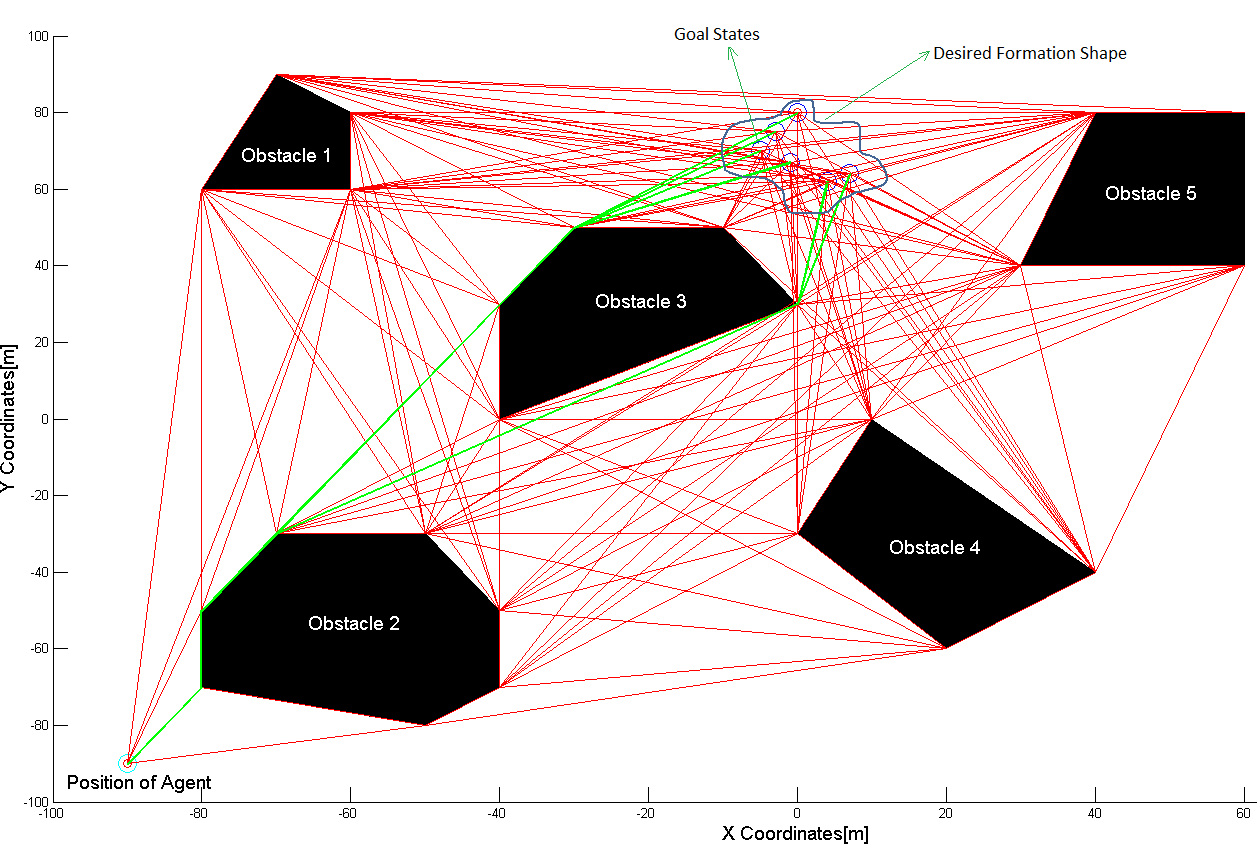
\includegraphics[scale = 0.40]{visgraph2}
\end{figure} 

Figure \ref{dijksttae_visibility} shows a simulation output executed with 5 workspace obstacles and 6 goal states in desired formation shape. In this algorithm, agent first calculates its own visibility graph by adding goal states $g_i \in G$ in graph as nodes. The visibility graph is illustrated with red edges in the figure. Then it calculates the shorthest paths to the goal states, which are given with green edges in the figure. We have used Dijkstra algorithm to compute the shortest path between two nodes in graph with multiple edges, each having a non-negative weight. In our work, the weights of the edges in $\gamma_{vis}$ , are calculated with the Euler distance between nodes in the workspace. Dijkstra algorithm is a tree search algorithm and time complexity of the original algorithm is $O(n^2)$ where $n$ is the number of the nodes in the graph. With the usage self balancing binary search tree, the algorithm requires $O(k+nlogn)$ time in the worst case where $k$ is the number of edges in the graph. The algorithm for the Dijkstra's is implemented as follows \cite{92}:
\newpage
	
\begin{algorithm}[H]
\KwData{$\gamma_{vis}$ , Position of the agent "$source$\_$ node$"}
\KwResult{Shortest Distance to goal states  $g_i \in G$ from the $source$\_$ node$ in $\gamma_{vis}$}
\For{<Each Vertex $v \subset \gamma_{vis}$>}
{		
Distance[v] := $\infty$ \;
Previous[v] := $undefined$ \;
}
Distance[$source$\_$ node$] :=0  \;
Q:= The set of all vertices $g_i \subset \gamma_{vis}$ \;
\While{<Q $\neq$ null>}
{
u:= Node in Q with smallest distance to $source$\_$ node$\;
remove u from Q\;
\For{<Each Neighbor v of u>}
{
alt:= Distance[u] + Cost Between u and v nodes\;
\If{alt<Distance[v]}
{
Distance[v] :=alt\;
Previous[v] :=u\;
}
}
}
return Previous[v]; \newline
\caption{DIJKSTRA$\_$ALGORITHM}
\end{algorithm}

In algorithm above $Distance[x]$ function call, calculates the total cost from the $source$\_$ node$ to the $x$ vertex, and $Previous[x]$ function call, returns the previous node in optimal path from $source$\_$ node$ . This algorithm calculates the shortest paths from the position of an agent to all available goal states. These cost values are used to assign the agents to the goal states by minimizing the total displacement.  

\paragraph{Collaborative Decision Process of Final Goal States}\hspace{0pt} \\
We have provided an algorithm to calculate the costs to the goal states $g_i \in G$ with the help of Visibility Graphs and Dijkstra's algorithm in previous sections. These costs are defined as displacements on the shortest paths to the goal states in the visibility graphs for each agent. In this project, our aim is to minimize the total displacement of the individuals while achieving the desired formation shape. For this purpose we have implemented an algorithm to minimize the overall displacement of whole swarm while achieving a formation shape. The problem related with this process can be defined as follows:

We have $n$ number of agents in our swarm and $n$ number of goal states $g_i \in G$ placed in desired formation shape. Each agent has reported their costs (i.e. minimum displacements) to reach each of these goal states and we have to implement an algorithm to assign the agents to these goal states while minimizing the total displacement of the swarm. This is a generalized assignment problem and we have used Hungarian algorithm which is a combinational optimization algorithm that solves this assignment problem. To implement this algorithm, a complete bipartite graph $G=(S,T,E)$ with $n \in S$ agents and $g_i \in T$ goal states is constructed.In this graph, each agent has a cost which is defined by the shortest path to the destination in the workspace for different goal points. 

\begin{figure}[H]
\centering
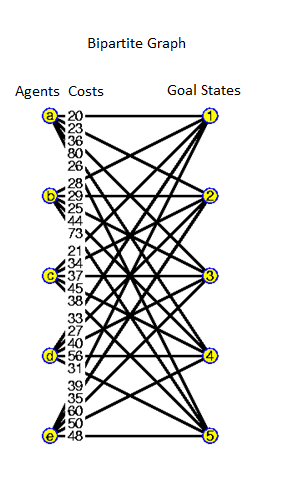
\includegraphics[width=.4\textwidth]{bipartite}
\caption{Sample Bipartite Graph Used in Assignment Problem \cite{102}}
\end{figure}

We have defiend a cost matrix  $C$ to implement the Hungarian algorithm. The dimensions of the cost matrix is $nxm$ in which each element represents the cost of assigning the goal state $m$ to the agent $n$.  Since we have equal number of agents and goal states, the cost matrix will be a square $nxn$ matrix.  The algorithm for the assignment process as follows:
	
\begin{algorithm}[H]
\KwData{Cost Matrix , $C$ }
\KwResult{Assignment Array of Agents to Goal States}
Label1  \;
\For{Each Row, $R$, in $C$ }{
Find the smallest element and subtract it from every element
}
Label 2  \; 
\If{A column,$K$, contains more than one zero}
{Repeat Label1 for each column, $K$}
Label 3  \; 

Select element in columns for which a distinct minimum weight has been determined and add to solution \newline
Label 4 \;
If it is not possible to reach the full solution, flag rows without solutions. Flag all columns in flagged rows that contain a zero. Flag all rows with a previously determined solution in previously flagged columns.
     
Label 5 \;
From elements remaining in flagged rows and unflagged rows, determine the element which has smallest value and assign this value to $\gamma$. Subtract $\gamma$  from every unflagged element and add  $\gamma$ to every element that has been flagged twice.
     
Label6 \;
Goto Label3 until full solution has been achieved. \newline    
\caption{HUNGARIAN$\_$ALGORITHM}
\end{algorithm}

Hungarian algorithm returns a vector of $nx1$ and each row in this vector represents the goal state that the related agent is assigned. With this assignment, the total cost (i.e. total displacement) of the swarm is minimized. 
\subsection{Mesh Quality Measurement}\hspace{0pt} \label{mesh_quality_ref}  \\
We have provided two different solutions to the shape partitioning problem. Bubble Packing method partitions the desired formation shape into goal states by distributing the bubbles which are representing our agents in the swarm. On the other hand, Randomized Fractals method randomly places the fractals in the desired shape and these fractals are representing our agents in the swarm. In this project one of our aims is to distribute the agents in the formation shape homogeneously. So it is useful to define a metric to compare the performances of these algorithms, i.e. a metric which represents how these methods homogeneously distribute the agents in the formation shape. One of the criterias we have used is topological mesh irregularity \cite{27} which is commonly used by mesh generation problems. To measure the topological mesh irregularity in our swarm, first we have constructed a Voronoi diagram with the nodes which are the center positions of the agents' coverage circles. Figure \ref{voronoi_voronoi} shows a simulation output about the final states of the agents in the desired formation shape. Centers of these coverage circles are used as positions of nodes while constructing the Voronoi diagram as illustrated in the right hand side of the figure.

\begin{figure}[H]
\caption{Voronoi Diagram Constructed with Final Positions of Agents} \label{voronoi_voronoi}
\centering
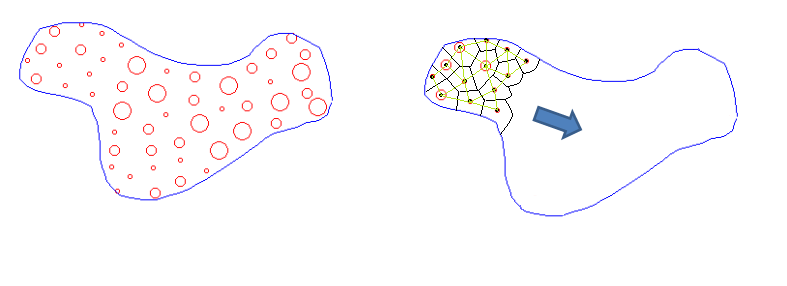
\includegraphics[scale = 0.70]{Artificial_Forces_Mesh_1}
\end{figure}

With the help of this Voronoi diagram, the topological mesh irregularity is defined by:

\begin{equation}
\epsilon _t = \frac{1}{n} \sum_{i = 0}^{n} |\gamma _i - D|
\end{equation}
	
where 

\begin{equation}
D = \left\{ \begin{array}{rl}
6                               &\mbox{ for triangles in Voronoi Diagram} \\
12                             &\mbox{ for tetrahedras in Voronoi Diagram}
\end{array} \right.
\end{equation}
	
and $\gamma _i$ represents the degree, or the number of neighboring nodes connected to the $i^{th}$ interior node, and $n$ represents the total number of interior nodes, i.e. the number of bubbles or fractals. In this implementation, topological mesh irregularity vanishes when all nodes have $D$ neighbors, but this ideal case is almost not possible in practical applications. Figure \ref{6komusulunode} shows a node with 6 neighbors in an example Voronoi diagram.
	
\begin{figure}[H]
\caption{A Node with 6 Neighbors} \label{6komusulunode}
\centering
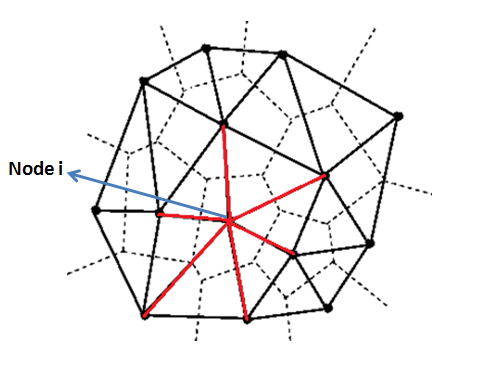
\includegraphics[scale = 0.70]{voronoi}
\end{figure}

Another metric we have used is geometrical mesh irregularity \cite{27}
With the help of the Voronoi diagram generated for the final state of the swarm, this irregularity is defined as \cite{27}:

\begin{equation}
\epsilon _g = \frac{1}{m} \sum_{i = 0}^{m} (A-\frac{r_i}{R_i})
\end{equation}

where
 
\begin{equation}
A = \left\{ \begin{array}{rl}
0.5                               &\mbox{ for triangles in Voronoi Diagram} \\
\sqrt{2/11}                   &\mbox{ for tetrahedras in Voronoi Diagram}
\end{array} \right.
\end{equation}
		
and $m$ represents the number of nodes, $r_i$ is the radii of inscribed circle of Voronoi cell belonging to node $i$ and $R_i$ is the radii of the circumscribing circle of Voronoi cell belonging to node $i$. Figure \ref{inscribe_circumscribe} shows inscribing and circumscribing circles of a Voronoi cell.
	
\begin{figure}[H]
\caption{Inscribing and Circumscribing Circle of a Voronoi Cell of Node i} \label{inscribe_circumscribe}
\centering
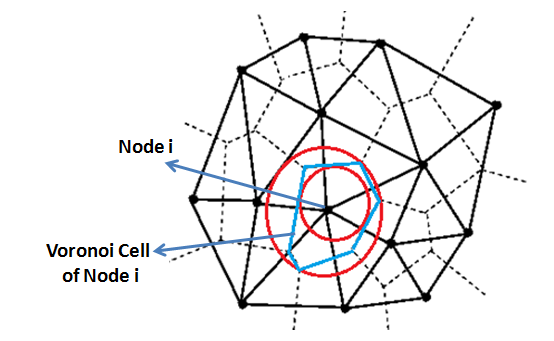
\includegraphics[scale = 0.70]{voronoi2}
\end{figure}

These irregularities show that how homogeneously the agents cover the desired formation shape in their final states. We expect to have lower values of irregularities for more homogeneous distributions. 
\subsection{Control System Design for Individual Agents}\hspace{0pt}\label{lqr_design}  \\ 
In shape partitioning methods we have implemented algorithms to calculate the potential goal states in desired formation shape. Then we have defined the assignment procedure of the agents to these goal states to minimize the total displacement of the agents in previous chapters. At this point, it is needed to implement navigation control laws for individual agents to make them reached to the goal states they have assigned. Since the environment is dynamically changing with lots of  mobile agents, it is very probable to have different assignments to these goal states at each execution step of formation control algorithm. Control system must react to these dynamically changing setpoints. For these purposes, we have designed a velocity controller with a large bandwidth as the inner loop of the control system and the outer loop is composed with a velocity setpoint generator. The block diagram for the proposed controller structure is presented in Figure \ref{Controller_ref}.

\begin{figure}[H]
\caption{General Scheme of the Control System} \label{Controller_ref}
\centering
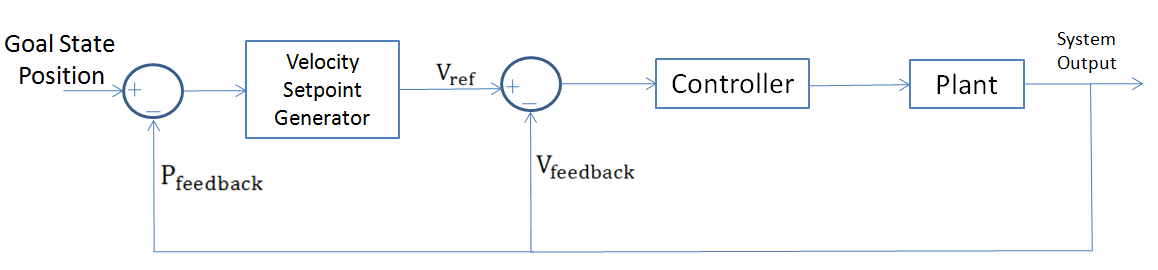
\includegraphics[scale = 0.45]{controller}
\end{figure}

In our implementation, velocity setpoint generator provides instant setpoints for the inner loop based on the current position of the agent and the desired goal state position.  This loop calculates the amplitude of the velocity setpoint proportional with the euclidian distance of agent to the desired goal state. The direction of this velocity setpoint vector has a bearing angle of the line segment drawn from the agent to the goal state. The additional terms discussed in Section \ref{shapepartition_ref} related with collision avoidance is added to this velocity setpoint. This generator saturates the amplitude of the setpoint vector with 0.5 [m/sec] to prevent the agents' travelling in the environment so fast. Figure \ref{velocity_sp_generation} shows the amplitude and the bearing angle to the destination goal state used by the velocity setpoint generator.

\begin{figure}[H]
\caption{Velocity Setpoint Generation} \label{velocity_sp_generation}
\centering
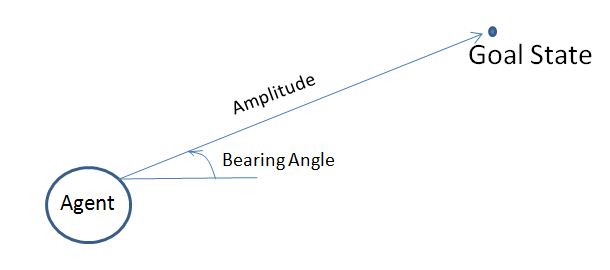
\includegraphics[scale = 0.50]{bearing}
\end{figure}

The inner loop is designed to track the velocity setpoint provided by the generator and it has a state feedback structure. The gains for the feedback states are calculated with LQR methodology. A simple mass, damper type second order linear system is used to provide a linear model for the controller design. The translational friction force is assumed to be linear with the velocity of each agent. Different mass and friction coefficients for heterogeneous mobile robots are used in control system design. To track the desired velocity setpoint, the model of the system is augmented with an artificial error state $e$,

\begin{equation} \label{dynamic_system}
\begin{bmatrix}
\dot{v} \\ \dot{e}
\end{bmatrix}
=
\begin{bmatrix}
-b/m & 0 \\
1 & 0
\end{bmatrix}
\begin{bmatrix}
v \\ e
\end{bmatrix}
+ \begin{bmatrix}
1/m \\ 0
\end{bmatrix}
F_{net} \hspace{0.5cm} and
\hspace{0.5cm}
y = \begin{bmatrix}
1 & 0
\end{bmatrix}
\begin{bmatrix}
v \\ e
\end{bmatrix}
\end{equation}

where $b$ is the linear friction force coefficient and $m$ is the mass, $v$  is the linear velocity of the agent and $e$ is the augmented error state which is the integral of the velocity state. Here the $v$ state is the stabilizing part of the controller and the $e$ error state is the tracker part of the controller. The state feedback gain, $K$, which minimizes the quadratic cost function of

\begin{equation}
J = \int_{t_o}^{t_1}(x^TQx + u^TRu) dt
\end{equation}

is calculated with help of $'lqr'$ function of MATLAB for the given system in Equation \ref{dynamic_system} with the gain matrices of 

\begin{equation}
Q = \begin{bmatrix}
q_1 & 0 \\ 0 & q_2
\end{bmatrix}
\hspace{0.3cm} and
\hspace{0.3cm}
R = r_1
\end{equation}

The parameters for the controller design are determined with the approach presented below,

\begin{equation}
q_1 = \frac{1}{t_1 (x_{1max})^2}; \hspace{0.1cm}
q_2 = \frac{1}{t_2 (x_{2max})^2}; \hspace{0.1cm} and \hspace{0.1cm}
r_1 = \frac{1}{ (u_{1max})^2}; \hspace{0.1cm}
\end{equation}

Here $t_i$  is the desired settling time for $x_i$ which is determined as 1.5 seconds for the velocity and 0.01 seconds for the integral state. The statement of $x_{imax}$ represents the expected maximum value of the state $i$ , which is defined 1 [m/sec] for the velocity state and 4 [m] for the error state. $u_{1max}$ represent the maximum allowable input signal which is defined as 3 [N]. The structure of the inner loop is illustrated in Figure \ref{innerloopref}

\begin{figure}[H]
\caption{Inner Loop Structure} \label{innerloopref}
\centering
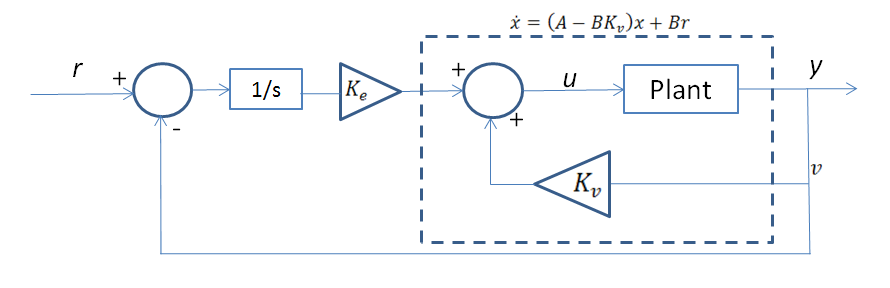
\includegraphics[scale = 0.50]{inner_loop}
\end{figure}

The error state ([m]) between the reference and the velocity feedback is integrated and multiplied with the error gain, and the velocity state is multiplied with the velocity gain. These two components generate the total control input of the system.  

\begin{figure}[H]
\caption{Step Response of the Closed Loop(Inner Loop)} \label{Stepresp}
\centering
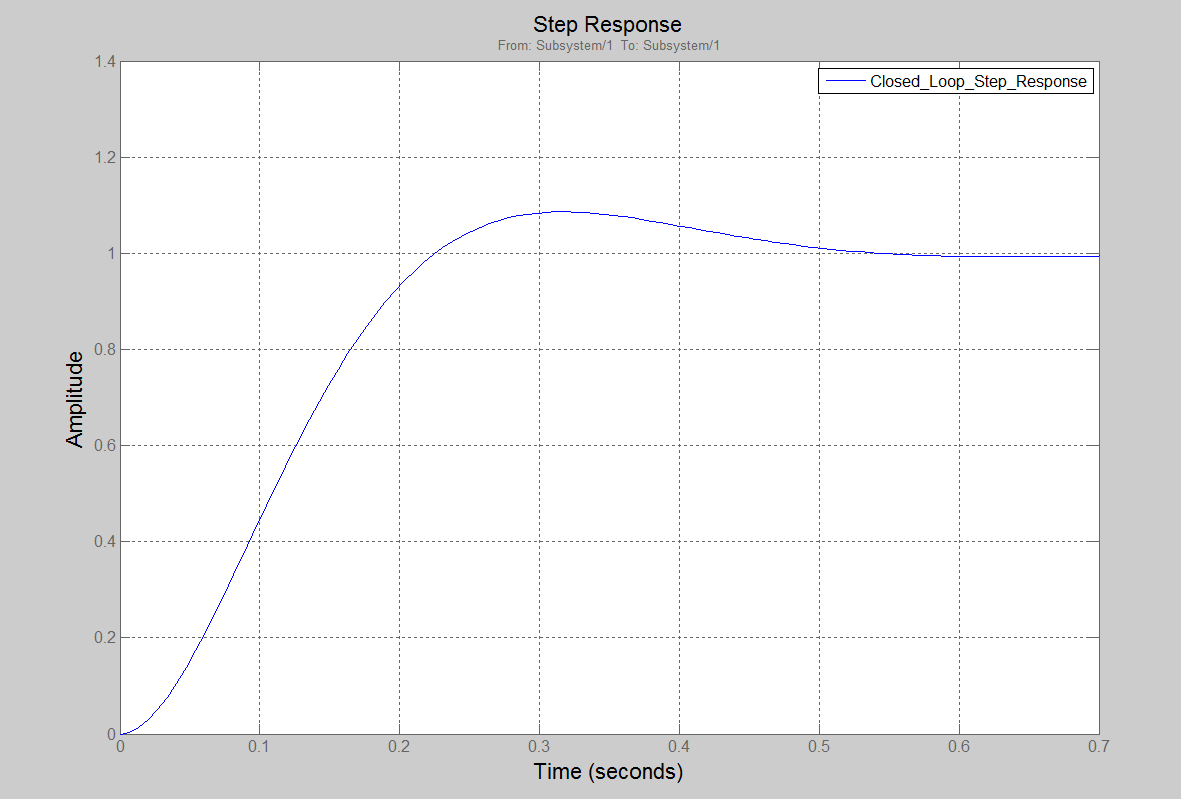
\includegraphics[scale = 0.40]{step_resp}
\end{figure}

According to the Figure \ref{Stepresp}, the settling time for the inner loop is around 0.5 seconds for a step input. System has an overshoot around $\%$10 .

\begin{figure}[H]
\caption{Closed Loop Bode Plot(Inner Loop)} \label{ClosedLoop}
\centering
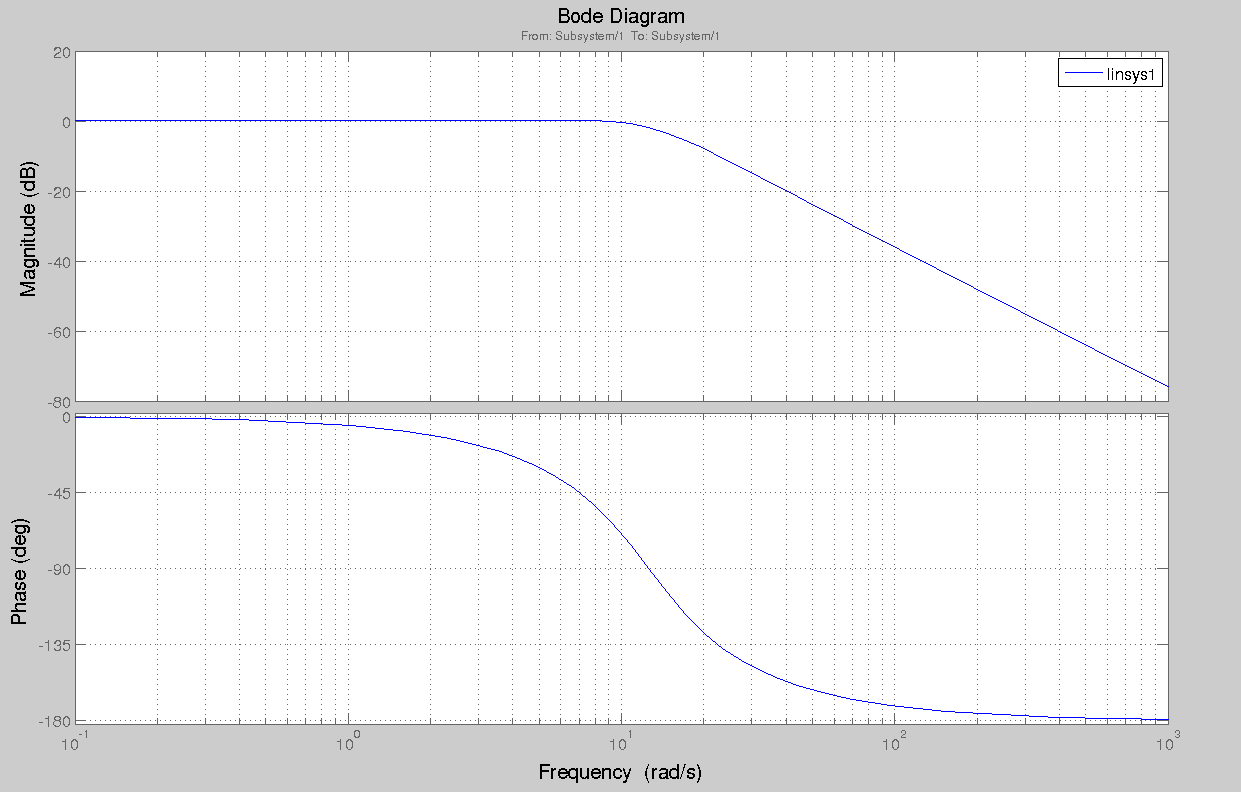
\includegraphics[scale = 0.30]{closed_loop}
\end{figure}

Figure \ref{ClosedLoop} shows the bode plot for the closed loop of the velocity controller. According to this figure inner loop which control the desired velocity setpoint has a bandwidth nearly 10 rad/sec.